% ==========================================================================
% Rapport final du projet RADAR
% Module M244 - Veille Technologique
% ENSA Tetouan - Cycle Ingenieur BDIA - Printemps 2026
% Auteurs : Bachirou Konate et Karamo Sylla
% Encadrant : Pr. Younes Wadiai
% ==========================================================================

\documentclass[12pt,a4paper,openany]{report}

% --- Encodage et langue ---------------------------------------------------
\usepackage[utf8]{inputenc}
\usepackage[T1]{fontenc}
\usepackage[french]{babel}
\usepackage{lmodern}

% --- Mise en page ---------------------------------------------------------
\usepackage[a4paper,top=2.5cm,bottom=2.5cm,left=3cm,right=2.5cm]{geometry}
\usepackage{setspace}
\onehalfspacing

% --- Couleurs (charte RADAR : Navy + Royal Blue + neutres chauds) ----------
\usepackage{xcolor}
\definecolor{ensaBlue}{HTML}{051C2C}      % RADAR Navy — titres, sections
\definecolor{ensaBlueLight}{HTML}{1F4868} % RADAR Navy-700 — sous-titres, libelle chapitre, en-tetes
\definecolor{ensaAccent}{HTML}{2251FF}    % RADAR Royal Blue — accent unique (filets, liens, encadres)
\definecolor{grayBox}{HTML}{FAF8F3}       % RADAR Cream — fonds d'encadres et de code
\definecolor{grayBorder}{HTML}{D4D4D8}    % hairline neutre

% --- Polices titres -------------------------------------------------------
\usepackage{titlesec}
\titleformat{\chapter}[display]
  {\normalfont\sffamily\Huge\bfseries\color{ensaBlue}\raggedright}
  {\sffamily\huge\color{ensaBlueLight}Chapitre \thechapter}
  {1ex}
  {\titlerule\vspace{1ex}\raggedright}
  [\vspace{0.5ex}\titlerule]
\titlespacing*{\chapter}{0pt}{-30pt}{20pt}
\titleformat{\section}
  {\normalfont\sffamily\Large\bfseries\color{ensaBlue}}
  {\thesection}{1em}{}
\titleformat{\subsection}
  {\normalfont\sffamily\large\bfseries\color{ensaBlueLight}}
  {\thesubsection}{1em}{}
\titleformat{\subsubsection}
  {\normalfont\sffamily\normalsize\bfseries\color{ensaBlueLight}}
  {\thesubsubsection}{1em}{}

% --- Graphiques et figures ------------------------------------------------
\usepackage{graphicx}
\graphicspath{{./}{images/}}
\usepackage{float}
\usepackage{pdfpages}
\usepackage{caption}
\captionsetup{font=small,labelfont={bf,color=ensaBlue},labelsep=period}
\usepackage{tikz}
\usetikzlibrary{shapes,arrows,positioning,fit,backgrounds,calc}

% --- Tableaux -------------------------------------------------------------
\usepackage{booktabs}
\usepackage{tabularx}
\usepackage{multirow}
\usepackage{array}
\usepackage{colortbl}
\newcolumntype{Y}{>{\raggedright\arraybackslash}X}

% --- Code source ----------------------------------------------------------
\usepackage{listings}
\lstdefinestyle{radarstyle}{
  backgroundcolor=\color{grayBox},
  basicstyle=\ttfamily\footnotesize,
  keywordstyle=\color{ensaBlue}\bfseries,
  commentstyle=\color{gray}\itshape,
  stringstyle=\color{ensaAccent},
  numbers=left,
  numberstyle=\tiny\color{gray},
  numbersep=8pt,
  frame=single,
  rulecolor=\color{grayBorder},
  breaklines=true,
  showstringspaces=false,
  tabsize=2,
  captionpos=b
}
\lstset{style=radarstyle}

% --- Encadres personnalises -----------------------------------------------
\usepackage[most]{tcolorbox}
\newtcolorbox{noteBox}[1][]{
  colback=grayBox,
  colframe=ensaBlueLight,
  fonttitle=\bfseries\sffamily\color{white},
  coltitle=white,
  colbacktitle=ensaBlueLight,
  title=Note,
  sharp corners,
  boxrule=0.5pt,
  #1
}
\newtcolorbox{decisionBox}[1][]{
  colback=grayBox,
  colframe=ensaAccent,
  fonttitle=\bfseries\sffamily\color{white},
  coltitle=white,
  colbacktitle=ensaAccent,
  title=Décision technique,
  sharp corners,
  boxrule=0.5pt,
  #1
}

% --- En-tetes et pieds de page --------------------------------------------
\usepackage{fancyhdr}
\pagestyle{fancy}
\fancyhf{}
\fancyhead[L]{\small\sffamily\color{ensaBlueLight}\nouppercase{\leftmark}}
\fancyhead[R]{\small\sffamily\color{ensaBlueLight}RADAR · M244}
\fancyfoot[C]{\thepage}
\renewcommand{\headrulewidth}{0.4pt}
\renewcommand{\footrulewidth}{0pt}

% --- Listes ---------------------------------------------------------------
\usepackage{enumitem}
\setlist{itemsep=2pt,topsep=4pt}

% --- Mise en colonnes pour la bibliographie -------------------------------
\usepackage{multicol}

% --- Liens et bibliographie ------------------------------------------------
\usepackage{hyperref}
\hypersetup{
  colorlinks=true,
  linkcolor=ensaBlue,
  urlcolor=ensaAccent,
  citecolor=ensaBlue,
  pdftitle={RADAR - Rapport final M244},
  pdfauthor={Bachirou Konate, Karamo Sylla},
  pdfsubject={Veille Technologique - ENSA Tetouan},
  bookmarksopen=true
}
\usepackage[french]{cleveref}

% --- Commande pour les figures a inserer plus tard ------------------------
\newcommand{\figurePlaceholder}[2]{%
  \begin{figure}[H]
    \centering
    \fbox{\parbox[c][4cm][c]{0.85\linewidth}{\centering\sffamily\color{gray}\itshape #2}}
    \caption{#1}
  \end{figure}
}

% Capture d'ecran : #1 = fichier, #2 = legende, #3 = label.
% Bornee en largeur ET hauteur (keepaspectratio) pour ne jamais deborder la page.
\newcommand{\screenshot}[3]{%
  \begin{figure}[H]
    \centering
    \includegraphics[width=\linewidth,height=0.45\textheight,keepaspectratio]{#1}
    \caption{#2}
    \label{#3}
  \end{figure}
}

\begin{document}

% =========================================================================
% PAGE DE GARDE
% =========================================================================
\begin{titlepage}
  \centering
  \vspace*{-3cm}

  % Logo ENSA agrandi et colle au bord superieur
  
\includegraphics[height=8cm]{logo_ensa.png}

  \vspace{-0.3cm}

  % Filets bleus encadrant les informations academiques (texte agrandi)
  {\color{ensaBlue}\rule{\linewidth}{1.2pt}}\\[10pt]
  {\sffamily\large\color{ensaBlue}\textbf{Cycle Ingénieur en Big Data et Intelligence Artificielle (BDIA)}}\\[5pt]
  {\sffamily\large\color{ensaBlueLight}Module M244 \; $\bullet$ \; Veille Technologique}\\[10pt]
  {\color{ensaBlue}\rule{\linewidth}{1.2pt}}

  \vspace{0.4cm}

  % Etiquette discrete au-dessus du titre
  {\sffamily\large\color{ensaBlueLight}\itshape Rapport de projet de fin de module}

  \vspace{0.8cm}

  % Titre principal dans un bloc bleu accentue, centre verticalement
  \begin{tcolorbox}[
    enhanced,
    colback=ensaBlue,
    colframe=ensaBlue,
    sharp corners,
    boxrule=0pt,
    left=15pt, right=15pt, top=28pt, bottom=28pt,
    width=\linewidth,
    drop fuzzy shadow=ensaBlueLight,
  ]
    \centering
    {\sffamily\fontsize{52}{56}\selectfont\bfseries\color{white} RADAR}\\[14pt]
    {\color{ensaAccent}\rule{4cm}{1pt}}\\[14pt]
    {\sffamily\Large\color{white} Plateforme de veille concurrentielle autonome}\\[6pt]
    {\sffamily\Large\color{white} propulsée par un agent IA}
  \end{tcolorbox}

  \vfill

  % Equipe et encadrant en deux colonnes
  \noindent
  \begin{minipage}[t]{0.48\linewidth}
    \raggedright\sffamily
    {\large\color{ensaBlue}\textbf{Réalisé par}}\\[4pt]
    {\color{ensaAccent}\rule{2.5cm}{1pt}}\\[8pt]
    \large KONATE BACHIROU\\[2pt]
    \large SYLLA KARAMO
  \end{minipage}\hfill
  \begin{minipage}[t]{0.48\linewidth}
    \raggedleft\sffamily
    {\large\color{ensaBlue}\textbf{Encadré par}}\\[4pt]
    {\color{ensaAccent}\rule{2.5cm}{1pt}}\\[8pt]
    \large Pr. Younes WADIAI
  \end{minipage}

  \vspace{1cm}

  % Annee universitaire dans un filet discret
  {\color{ensaBlueLight}\rule{0.4\linewidth}{0.4pt}}\\[8pt]
  {\sffamily\large\color{ensaBlue}\textbf{Année universitaire 2025 -- 2026}}

\end{titlepage}

% =========================================================================
% REMERCIEMENTS
% =========================================================================
\chapter*{Remerciements}
\addcontentsline{toc}{chapter}{Remerciements}
\thispagestyle{empty}

\vspace{2cm}

Nous adressons nos remerciements les plus sincères au Pr. Younes Wadiai, enseignant du module M244 Veille Technologique à l'École Nationale des Sciences Appliquées de Tétouan, pour la rigueur de son enseignement et la clarté de la méthodologie qu'il nous a transmise. Sans le cadre conceptuel du cycle de veille, des grilles d'analyse SWOT et PESTEL, de la grille CRAAP et des signaux faibles que nous avons reçus en cours, ce projet n'aurait pu prendre la forme d'un produit opérationnel. Nous lui sommes également reconnaissants pour la liberté qu'il nous a laissée dans le choix d'un sujet ambitieux, et pour son ouverture d'esprit face à une réalisation qui croise sa spécialité avec l'intelligence artificielle générative.

\vfill

% =========================================================================
% RESUME
% =========================================================================
\chapter*{Résumé}
\addcontentsline{toc}{chapter}{Résumé}

Ce rapport présente RADAR, un outil pensé pour les entreprises qui veulent savoir chaque semaine ce que font leurs concurrents sans y passer plusieurs heures chaque matin.

L'utilisation est directe. On indique le nom de son entreprise et celui de ses concurrents principaux, et RADAR s'occupe du reste. Chaque semaine, il parcourt le web pour repérer les nouvelles informations qui touchent ces concurrents : changements de prix, recrutements importants, lancements de produits, levées de fonds, campagnes de communication. L'intelligence artificielle qui pilote l'outil lit ces informations, fait le tri entre celles qui sont fiables et celles qui ne le sont pas, et ne retient que ce qui mérite vraiment l'attention.

Chaque lundi, un compte-rendu structuré est mis à disposition dans l'application, sur la page Rapports. On y trouve un résumé rapide des mouvements de la semaine, une analyse des forces et faiblesses de l'entreprise face à la concurrence, une lecture des grandes tendances de son secteur, une liste d'indices qui annoncent des évolutions à venir, et des recommandations classées par ordre d'importance. Le rapport se consulte directement dans le tableau de bord en ligne et s'exporte en PDF pour être téléchargé, archivé et partagé avec les membres de la direction lors des réunions ou comme livrable client.

% =========================================================================
% TABLE DES MATIERES
% =========================================================================
\tableofcontents
\listoffigures
\listoftables

% =========================================================================
% LISTE DES ACRONYMES
% =========================================================================
\chapter*{Liste des acronymes et abréviations}
\addcontentsline{toc}{chapter}{Liste des acronymes et abréviations}

\begin{description}[leftmargin=3.5cm,style=nextline]
  \item[API] Application Programming Interface
  \item[BDIA] Big Data et Intelligence Artificielle
  \item[CRAAP] Currency, Relevance, Authority, Accuracy, Purpose
  \item[CRUD] Create, Read, Update, Delete
  \item[ENSA] École Nationale des Sciences Appliquées
  \item[ERD] Entity Relationship Diagram
  \item[HTTP] Hypertext Transfer Protocol
  \item[ICP] Ideal Customer Profile
  \item[JSON] JavaScript Object Notation
  \item[LLM] Large Language Model
  \item[M244] Code du module Veille Technologique
  \item[MVP] Minimum Viable Product
  \item[ORM] Object Relational Mapping
  \item[OAuth] Open Authorization
  \item[PDF] Portable Document Format
  \item[PESTEL] Politique, Économique, Sociologique, Technologique, Environnemental, Légal
  \item[PME] Petite et Moyenne Entreprise
  \item[PRD] Product Requirements Document
  \item[RGPD] Règlement Général sur la Protection des Données
  \item[SaaS] Software as a Service
  \item[SSO] Single Sign-On
  \item[SWOT] Strengths, Weaknesses, Opportunities, Threats
  \item[TPM] Tokens Per Minute
  \item[UI] User Interface
\end{description}

% =========================================================================
% CHAPITRE 1 - INTRODUCTION ET VUE D'ENSEMBLE
% =========================================================================
\chapter{Introduction et vue d'ensemble}
\label{chap:introduction}

\section{Introduction générale}
\label{sec:introduction-generale}

Ce rapport rend compte du travail mené pour concevoir et développer RADAR, dans le cadre du module M244 Veille Technologique du cycle ingénieur Big Data et Intelligence Artificielle de l'École Nationale des Sciences Appliquées de Tétouan.

Le module M244 forme les futurs ingénieurs aux pratiques de la veille stratégique : cerner un besoin d'information, collecter, évaluer les sources, analyser avec les grilles SWOT et PESTEL, repérer les signaux faibles, puis diffuser des résultats exploitables. Pour le valider, il faut un projet de fin de semestre qui prouve qu'on maîtrise ces notions sur un cas concret.

Plutôt que de mener une veille sur une seule entreprise, nous avons choisi de livrer un logiciel : une plateforme qui automatise tout le cycle de veille, pour n'importe quelle entreprise, en s'appuyant sur les grands modèles de langage récents. Trois raisons à ce choix. D'abord, transformer chaque notion du cours en une brique technique qu'on peut réellement tester. Ensuite, aboutir à un outil utilisable sur le terrain, y compris par un dirigeant de PME ou un consultant sans bagage technique. Enfin, repartir du semestre avec une réalisation concrète à présenter en entretien, que ce soit en stratégie, en data ou en IA appliquée.


\section{Problématique et besoin identifié}
\label{sec:problematique}

Toute entreprise qui évolue dans un marché concurrentiel doit savoir ce que font ses rivaux. Les dirigeants de PME, les responsables stratégie et les consultants le savent bien : un concurrent qui ajuste ses prix, recrute en masse, lève des fonds ou refond son offre, c'est une information qui peut faire basculer une décision. Le problème n'est pas que ces informations manquent, au contraire, elles sont largement publiques. Le problème, c'est que dans une organisation de taille moyenne, personne n'a le temps de les collecter chaque semaine, de les recouper, de les évaluer puis de les mettre en forme.

En pratique, la veille concurrentielle prend rarement une forme aboutie dans les PME et même dans les grandes entreprises. La situation la plus fréquente : aucune routine formalisée, la direction se contente du bouche-à-oreille sectoriel et de ce qui remonte sur LinkedIn. Variante un peu plus mature : un collaborateur dédie une heure ou deux chaque matin à naviguer sur les sites concurrents, scroller les réseaux, lire la presse économique, et consigne ce qu'il en retient dans un tableur sans grille d'analyse. Cas plus rare : l'entreprise s'abonne à Similarweb, SEMrush ou Crayon, mais finit par constater que ces outils répondent surtout à des besoins SEO et marketing, pas à une veille stratégique au sens du cycle enseigné en M244.

Les mêmes faiblesses reviennent dans ce mode de fonctionnement. La découverte est tardive : un changement de prix ou une levée de fonds remonte par la presse des semaines après les faits. Les sources ne sont pas évaluées, si bien que rumeurs et informations confirmées se retrouvent sur le même plan. Rien n'est mis en forme en SWOT ou en PESTEL, ce qui complique tout raisonnement sur les axes stratégiques. Les signaux faibles, ces indices précoces et dispersés qui annoncent un mouvement de fond, passent inaperçus. Et il n'existe aucune mémoire centralisée : chaque revue repart de zéro.

Le besoin est simple à formuler : disposer chaque semaine d'une synthèse concurrentielle prête à lire, fondée sur la méthodologie M244, sans qu'un humain ait à la produire à la main. L'outil doit couvrir le cycle complet, de la collecte à la diffusion en passant par l'analyse, et ne remonter que des informations vérifiées et recoupées. C'est précisément ce que fait RADAR.

\section{Objectifs et solution}
\label{sec:objectifs-solution}

L'objectif principal est simple : une plateforme qui déroule seule le cycle de veille, de la collecte jusqu'à la livraison du rapport hebdomadaire. Cinq objectifs opérationnels en découlent.

Automatiser la collecte web sans se faire bloquer par les protections anti-bot, en passant par un fournisseur de recherche pensé pour les agents. Évaluer chaque source avec la grille CRAAP avant de l'utiliser, pour que la fiabilité de ce qui remonte reste traçable. Produire des SWOT et des PESTEL qui tiennent la route face à un examen critique. Détecter les signaux faibles, ces indices précoces d'une évolution du secteur. Et livrer le tout dans un tableau de bord sobre, où chaque rapport se consulte, se télécharge en PDF et se partage.

La solution repose sur un agent d'intelligence artificielle piloté par OpenClaw, un runtime open source qui exécute des compétences décrites au format Markdown. L'agent RADAR en mobilise huit. Deep Research dresse le profil de l'entreprise utilisatrice à l'inscription, en dehors du cycle hebdomadaire. L'orchestrateur coordonne le reste. Le collecteur interroge Tavily pour ramener des sources fraîches sur chaque concurrent ; l'évaluateur leur attribue un score CRAAP ; deux analystes produisent la PESTEL puis la SWOT ; un détecteur cherche les signaux faibles ; et un rédacteur met tout en forme dans un rapport narratif. L'orchestrateur enchaîne ces compétences avec le mécanisme de sous-sessions d'OpenClaw, ce qui isole les contextes et garde la consommation de tokens sous contrôle.

Côté utilisateur (dirigeant de PME ou de grand groupe, consultant, étudiant en stratégie), tout passe par une application web sous Next.js 16. À l'inscription, il donne le nom de son entreprise et son site, ajoute ses concurrents prioritaires et choisit ses axes de surveillance. Le moteur agent prend ensuite le relais : chaque lundi à six heures, un cron lance l'orchestrateur, qui déroule toute la chaîne, écrit les résultats en base via les routes internes et met le rapport à disposition. La consultation se fait dans un tableau de bord : feed des alertes, grilles SWOT et PESTEL, timeline des mouvements détectés, signaux faibles. Sur la page Rapports, l'utilisateur ouvre le rapport, le télécharge en PDF et le partage en comité de direction ou comme livrable client.


\section{Méthodologie projet et planification}
\label{sec:methodologie}

Nous avons travaillé en cycles courts, d'une à deux semaines, dans l'esprit du développement itératif et du Lean Startup. Plutôt que de tout spécifier avant d'écrire la première ligne de code, chaque cycle se terminait par quelque chose de montrable : un composant assemblé ou une série de tests d'intégration. C'est ce qui nous a permis d'encaisser sans trop de casse les décisions qu'on ne pouvait pas voir venir, comme l'abandon de GPT-4o pour DeepSeek V4 Pro (limites de tokens par minute) ou le passage de DuckDuckGo à Tavily (blocage des rafales de requêtes).

Les outils mobilisés pour la coordination et le développement sont résumés dans le tableau \ref{tab:outils-projet}.

\begin{table}[H]
  \centering
  \caption{Outils de travail et de coordination utilisés sur le projet RADAR}
  \label{tab:outils-projet}
  \small
  \begin{tabularx}{\linewidth}{lY}
    \toprule
    \textbf{Catégorie} & \textbf{Outils retenus} \\
    \midrule
    Versionnement et collaboration & Git, GitHub (branches \texttt{feature/agent} et \texttt{feature/web}, pull requests) \\
    Gestion du monorepo & pnpm 10, Turborepo \\
    Documentation interne & Fichiers Markdown versionnés \\
    Conteneurisation & Docker, Docker Compose, image officielle \texttt{ghcr.io/openclaw/openclaw:latest} \\
    Tests d'intégration & Mock API HTTP en Node.js qui simule les routes Next.js côté agent \\
    Éditeur de code & Visual Studio Code, LaTeX (pour le rapport), ESLint, Prisma \\
    Communication équipe & WhatsApp pour le quotidien, sessions de travail synchrones le week-end \\
    \bottomrule
  \end{tabularx}
\end{table}

La planification du projet s'est étalée entre mars et juin 2026, en suivant l'enchaînement de phases présenté dans la figure \ref{fig:gantt-projet}.

\begin{figure}[H]
  \centering
  
\includegraphics[width=\linewidth]{planification_radar.png}
  \caption{Diagramme de Gantt de la planification du projet RADAR}
  \label{fig:gantt-projet}
\end{figure}

\section{Cahier des charges simplifié}
\label{sec:cahier-charges}

RADAR n'est pas qu'un exercice scolaire : nous l'avons pensé comme une offre qu'on pourrait facturer à un client. Le tableau \ref{tab:cahier-charges} reprend le cahier des charges de la version 1 dans cette logique.

\begin{table}[H]
  \centering
  \caption{Cahier des charges synthétique de RADAR V1}
  \label{tab:cahier-charges}
  \small
  \begin{tabularx}{\linewidth}{lY}
    \toprule
    \textbf{Rubrique} & \textbf{Engagement} \\
    \midrule
    Besoin client & Disposer chaque semaine d'un rapport de veille concurrentielle structuré, sans intervention manuelle, couvrant entre un et dix concurrents nommés par l'utilisateur. \\
    Fonctionnalités clés & Inscription guidée avec enrichissement automatique du profil entreprise (Deep Research), cycle de veille hebdomadaire déclenché par cron, dashboard temps réel, consultation et export PDF des rapports. \\
    Contraintes techniques & Hébergement Docker mutualisé ou self-hosted (VPS Hetzner CX21), dépendance externe à DeepSeek (modèle LLM) et Tavily (recherche web), réseau interne entre les services, persistance PostgreSQL. \\
    Indicateurs de succès & Rapport produit chaque semaine, le lundi avant 7h00, sources évaluées CRAAP avec score moyen supérieur à 14 sur 20, recoupement minimum à deux sources indépendantes pour chaque alerte, taux d'échec inférieur à 5 pour cent par cycle. \\
    Délai de livraison & Une version opérationnelle déployée sur VPS au plus tard une semaine avant la soutenance, c'est-à-dire mi-juin 2026. \\
    Ressources mobilisées & Deux développeurs étudiants en cycle ingénieur, environ vingt heures hebdomadaires chacun sur la durée du semestre. \\
    Résultats attendus & Une plateforme utilisable en mode démonstration pour le jury, un rapport documenté, un dépôt Git public, et la capacité à soutenir une démonstration en direct sur un compte test. \\
    \bottomrule
  \end{tabularx}
\end{table}

Ce cahier des charges servira de référence tout au long du rapport : chaque choix technique présenté dans les chapitres suivants pourra être confronté aux engagements pris ici, et le chapitre 7 établira un bilan honnête de ce qui a été tenu et de ce qui reste à finaliser.

% =========================================================================
% CHAPITRE 2 - ETAT DE L'ART
% =========================================================================
\chapter{État de l'art}
\label{chap:etat-art}

Ce chapitre replace RADAR dans deux contextes qui le précèdent : la veille stratégique comme discipline, et les agents IA comme technologie. Il reste court : l'idée est surtout de situer notre solution et de la distinguer de ce qui existe déjà sur le marché.

\section{Concepts fondateurs de la veille stratégique}
\label{sec:concepts-veille}

La veille stratégique a été formalisée dans la littérature francophone par Humbert Lesca. Le module M244 du Pr. Younes Wadiai l'enseigne à travers quatre concepts, que nous avons repris tels quels dans le moteur RADAR.

Le \textbf{cycle de veille} en cinq étapes (identification des besoins, collecte, analyse et traitement, diffusion et exploitation, mise à jour continue) sert de colonne vertébrale au pipeline : chaque compétence du moteur couvre un segment du cycle.

Pour évaluer les sources, nous utilisons la \textbf{grille CRAAP} (Currency, Relevance, Authority, Accuracy, Purpose), proposée par Sarah Blakeslee en 2004. Chaque critère vaut quatre points, soit un score sur vingt. L'Évaluateur le calcule pour chaque source, et un seuil de cinq sur vingt déclenche le filtrage.

L'analyse stratégique mobilise les grilles \textbf{SWOT} (forces et faiblesses internes, opportunités et menaces externes) et \textbf{PESTEL} (six dimensions : politique, économique, sociologique, technologique, environnementale, légale). RADAR produit la grille SWOT comme la grille PESTEL au rythme hebdomadaire.

Enfin, RADAR détecte les \textbf{signaux faibles} théorisés par Igor Ansoff en 1975 dans \textit{Managing Strategic Surprise by Response to Weak Signals}. La compétence dédiée croise les sources mineures (forums, blogs, offres d'emploi) et majeures sur une fenêtre glissante de trente jours stockée en base PostgreSQL, pour faire émerger des récurrences qui annoncent un mouvement de fond.

\section{Panorama des outils de veille existants}
\label{sec:panorama-outils}

Le marché de la veille concurrentielle est dense mais éclaté. Les outils les plus connus répondent en fait à des besoins très différents, et la plupart ne couvrent pas la veille stratégique méthodologique au sens du M244. Le tableau \ref{tab:benchmark-outils} récapitule les solutions que nous avons regardées au moment du cadrage.

\begin{table}[H]
  \centering
  \caption{Panorama comparé des principaux outils de veille concurrentielle}
  \label{tab:benchmark-outils}
  \small
  \begin{tabularx}{\linewidth}{lYY}
    \toprule
    \textbf{Outil} & \textbf{Cœur métier} & \textbf{Limite par rapport à RADAR} \\
    \midrule
    Similarweb & Mesure du trafic web, classement par catégorie, sources d'audience & Aucune analyse SWOT ni PESTEL, pas de détection de signaux faibles, orienté SEO et marketing \\
    SEMrush & Positionnement de mots-clés, backlinks, suivi de la présence digitale & Même limite : centré sur le SEO, ne couvre pas la veille stratégique \\
    Crayon & Veille concurrentielle enterprise avec battlecards et alerting & Très orienté sales enablement grand compte, prix prohibitif pour une PME \\
    Mention & Social listening, mentions de marque, sentiment & Pas de cadre méthodologique, ne produit pas de grille d'analyse \\
    Brandwatch & Social listening grand compte avec analytics avancés & Même remarque, plus la barrière du prix \\
    Google Alerts & Notification de nouveautés à partir de mots-clés & Beaucoup trop bruyant, aucune évaluation des sources, pas de structuration \\
    Feedly & Agrégateur de flux RSS avec couche IA optionnelle & Centré sur la lecture, ne génère pas de synthèse stratégique \\
    \bottomrule
  \end{tabularx}
\end{table}

Aucun ne prend le cycle M244 comme fil conducteur. C'est là que RADAR se place : produire chaque semaine des livrables stratégiques structurés par une méthode explicite, pour des PME et des consultants indépendants qui n'ont ni le budget ni le besoin des suites enterprise.

\section{Évolution des agents IA autonomes}
\label{sec:agents-ia}

En intelligence artificielle, le terme \textit{agent} désigne depuis longtemps un programme capable de percevoir son environnement et d'agir pour atteindre un objectif. Tout a changé en 2023 avec les grands modèles de langage : le moteur de raisonnement n'est plus une suite de règles écrites à la main, mais un LLM auquel on donne accès à des outils externes et à une mémoire de travail. AutoGPT, publié en avril 2023, a popularisé cette approche, suivi par des frameworks plus aboutis comme LangChain et son évolution LangGraph.

Les architectures actuelles reposent sur quatre briques : un LLM comme moteur de raisonnement, des outils pour agir au-delà du texte (recherche web, lecture de fichiers, exécution de code), une mémoire à court et long terme, et une boucle de contrôle qui décide quand mobiliser chaque outil.

OpenClaw, le runtime que nous avons retenu pour RADAR, intègre ces briques dans un seul binaire compatible avec l'API OpenAI Chat Completions. Les comportements d'un agent se décrivent dans des fichiers Markdown \texttt{SKILL.md}, lisibles et modifiables sans recompilation. La fonction \texttt{sessions\_spawn} crée des sous-sessions isolées indispensables à un pipeline séquentiel, le cron natif gère le déclenchement hebdomadaire, et les outils \texttt{web\_search}, \texttt{web\_fetch} et \texttt{browser} sont disponibles sans configuration. Face à un paysage mouvant (Claude Agent SDK, Mastra, LangGraph, plateformes hébergées), notre choix repose sur le caractère open source du code, la compatibilité native avec l'API OpenAI qui ouvre la porte à tous les modèles disponibles dans cette interface, et la lisibilité immédiate du format SKILL.md.

\section{Positionnement de RADAR}
\label{sec:positionnement-radar}

RADAR ne cherche pas à remplacer Similarweb, ni à faire l'agrégateur de flux, le social listener ou le framework d'agents généraliste. Son terrain est plus étroit : automatiser le cycle de veille M244 pour des PME et des consultants, en transformant chaque notion du cours en une fonctionnalité visible dans le produit.

Cette spécialisation est à la fois la force et la limite du projet. Force, parce qu'elle assure une cohérence méthodologique que les outils généralistes n'ont pas : chaque source collectée est évaluée par CRAAP, chaque alerte est recoupée, chaque rapport suit la structure attendue par le cours. Limite, parce qu'elle restreint le périmètre fonctionnel et nous oblige à laisser de côté des sujets adjacents comme la veille brevet, la veille réglementaire ou la surveillance de la réputation en ligne. Ces sujets pourraient faire l'objet d'extensions, dont nous discutons dans les perspectives du chapitre 7.

% =========================================================================
% CHAPITRE 3 - ARCHITECTURE DE RADAR
% =========================================================================
\chapter{Architecture de RADAR}
\label{chap:architecture}

Ce chapitre décrit l'architecture technique de RADAR : comment les composants s'articulent, quelles décisions ont structuré la conception, quelle stack nous avons retenue et comment nous isolons les sessions utilisateur.

\section{Schéma global du système}
\label{sec:schema-global}

RADAR fonctionne sur trois services Docker indépendants qui collaborent via un réseau interne. Le premier est l'application web bâtie sur Next.js qui sert d'interface utilisateur et de couche de persistance. Le deuxième est le moteur agent OpenClaw qui exécute les huit compétences spécialisées. Le troisième est la base de données PostgreSQL qui stocke profils, sources, analyses et rapports. La figure \ref{fig:archi-globale} schématise cette topologie.

\begin{figure}[H]
  \centering
  
\includegraphics[width=\linewidth]{schema_global_radar.png}
  \caption{Architecture globale de RADAR}
  \label{fig:archi-globale}
\end{figure}

Le flux nominal d'un cycle de veille suit toujours la même séquence. Un cron déclenche l'orchestrateur chaque lundi à six heures du matin, ou un bouton dans le dashboard utilisateur peut le déclencher à la demande. L'orchestrateur lit le profil utilisateur passé en paramètre du message initial, puis enchaîne les sous-sessions via \texttt{sessions\_spawn}. Chaque sous-session exécute une compétence : collecte, évaluation, analyses, détection des signaux faibles, rédaction. Après chaque étape, la compétence envoie ses résultats à l'application web via une route interne dédiée, et retourne son livrable à l'orchestrateur pour alimenter l'étape suivante. Une fois le cycle terminé, le rapport final est marqué comme achevé dans la base et devient consultable par l'utilisateur dans l'application, sur la page Rapports.

\section{Choix d'architecture clés}
\label{sec:choix-architecture}

Cinq décisions structurantes ont orienté la conception. Nous les listons ici parce qu'elles conditionnent tous les chapitres suivants.

\begin{decisionBox}[title={Décision 1 : un seul agent OpenClaw avec huit compétences, et non huit agents distincts}]
OpenClaw permet de définir plusieurs agents dans un même processus. Chaque agent dispose alors de son propre modèle, de ses propres outils, de sa propre mémoire. Cette approche multi-agent a un coût : la communication entre agents passe par des messages externes, ce qui complique l'orchestration et augmente la latence. Nous avons préféré une architecture simple : un seul agent (l'agent \texttt{main}) qui charge huit compétences au format SKILL.md. L'orchestration interne se fait alors via \texttt{sessions\_spawn}, qui crée des sous-sessions isolées du même agent. Cette décision a été validée après lecture de la documentation OpenClaw : \texttt{sessions\_spawn} ne sait pas cibler un autre agent, il opère sur l'agent courant.
\end{decisionBox}

\begin{decisionBox}[title={Décision 2 : communication agent vers web via HTTP interne, sans signature HMAC}]
Les architectures de webhook classiques exigent une signature HMAC pour authentifier l'expéditeur. RADAR utilise un réseau Docker interne fermé : seuls les conteneurs déclarés dans le même \texttt{docker-compose.yml} peuvent atteindre les routes \texttt{/api/internal/*}. Cette isolation réseau rend la signature HMAC superflue en V1. Si le produit devait passer en multi-tenant hébergé sans isolation réseau, l'ajout d'une couche HMAC serait la première chose à faire ; nous l'avons documenté comme dette technique connue.
\end{decisionBox}

\begin{decisionBox}[title={Décision 3 : modèle LLM DeepSeek V4 Pro, et non GPT-4o ni Claude Opus}]
Notre premier prototype utilisait GPT-4o. Il atteignait rapidement la limite de trente mille tokens par minute du Tier 1 OpenAI, ce qui bloquait la compétence Deep Research qui consomme à elle seule près de trente mille tokens sur le dernier appel. DeepSeek V4 Pro offre un contexte d'un million de tokens, une limite de débit élastique et un coût dix-sept fois inférieur à celui de GPT-4o, tout en restant compatible avec l'API OpenAI Chat Completions qu'OpenClaw exploite. La dégradation de qualité par rapport à Claude Opus 4.7 sur les analyses SWOT et PESTEL est restée acceptable lors des tests d'intégration.
\end{decisionBox}

\begin{decisionBox}[title={Décision 4 : Tavily comme provider primaire de recherche web, DuckDuckGo en fallback}]
DuckDuckGo est gratuit et fonctionne sans clé API, ce qui en a fait notre premier choix. Mais le moteur applique une détection de bot agressive sur les rafales de requêtes, et la compétence Collecteur en émet typiquement quinze à vingt par cycle. Tavily, conçu pour les agents IA, retourne le contenu complet des pages (pas seulement les URL), n'applique pas de détection de rafales sur le free tier et offre mille requêtes par mois. La compétence Deep Research peut continuer à utiliser DuckDuckGo car ses requêtes sont espacées dans le temps, mais le Collecteur passe par Tavily.
\end{decisionBox}

\begin{decisionBox}[title=Décision 5 : cron OpenClaw natif et orchestrateur sans persistance propre]
OpenClaw embarque un scheduler cron natif qui déclenche un message initial vers un agent à l'heure configurée. Plutôt que d'ajouter une couche de scheduling externe comme pg-boss ou node-cron du côté Next.js, nous nous sommes contentés du cron OpenClaw. L'orchestrateur lui-même ne maintient pas d'état persistant : chaque cycle est indépendant et l'intégralité de la traçabilité remonte dans la base PostgreSQL via les routes internes. Cette simplicité réduit le nombre de composants à opérer en production.
\end{decisionBox}

\section{Stack technique justifiée}
\label{sec:stack-technique}

Le tableau \ref{tab:stack} résume la stack technique retenue et les raisons de chaque choix.

\begin{table}[H]
  \centering
  \caption{Stack technique de RADAR et justification de chaque brique}
  \label{tab:stack}
  \small
  \begin{tabularx}{\linewidth}{lYY}
    \toprule
    \textbf{Couche} & \textbf{Technologie} & \textbf{Raison du choix} \\
    \midrule
    Frontend & Next.js 16, React 19, Tailwind CSS 4 & Standard de l'écosystème JavaScript, support natif du SSR et des Server Actions, communauté large \\
    Authentification & Better-Auth & Support Next.js App Router, OAuth Google intégré, sessions DB-backed \\
    Base de données & PostgreSQL 17 & Robustesse, support JSONB pour les structures semi-structurées des analyses, gratuit \\
    ORM & Prisma 6 & Génération de types TypeScript à partir du schéma, migrations versionnées \\
    Runtime Node & Node 24 & Dernière LTS au moment du projet, performances améliorées \\
    Monorepo & pnpm 10, Turborepo & Gestion partagée des dépendances, cache de build entre packages \\
    Moteur agent & OpenClaw (image \texttt{ghcr.io/openclaw/openclaw:latest}) & Open source, format SKILL.md lisible, sessions\_spawn natif \\
    Modèle LLM & DeepSeek V4 Pro (\texttt{deepseek/deepseek-v4-pro}) & Contexte 1M tokens, coût dix-sept fois inférieur à GPT-4o, compatible API OpenAI \\
    Recherche web & Tavily (primaire), DuckDuckGo (fallback) & Tavily conçu pour agents IA, pas de bot detection, contenu complet retourné \\
    Conteneurisation & Docker, Docker Compose & Standard d'industrie, environnement reproductible local et production \\
    Hébergement V1 & Hetzner Cloud CX21 & Coût maîtrisé (~4 EUR par mois), serveurs allemands conformes RGPD \\
    \bottomrule
  \end{tabularx}
\end{table}

Nous avons choisi cette stack en visant deux choses à la fois : un coût d'exploitation minimal, parce que le projet n'a aucun budget commercial, et la maintenabilité, parce qu'un développeur extérieur doit pouvoir reprendre le code. Chaque brique est éprouvée et largement utilisée.

\section{Sécurité et isolation des sessions utilisateur}
\label{sec:securite}

La sécurité d'une plateforme qui agrège des données concurrentielles pour plusieurs clients mériterait un chapitre à elle seule. RADAR reste un MVP, mais nous avons quand même pris plusieurs précautions dès la conception, pour ne pas accumuler une dette de sécurité difficile à rattraper ensuite.

\textbf{Isolation réseau.} Les trois services Docker (Next.js, OpenClaw, PostgreSQL) communiquent uniquement sur un réseau privé déclaré dans le \texttt{docker-compose.yml}. Seuls les ports HTTPS de l'application web sont exposés vers l'extérieur. OpenClaw n'est jamais accessible depuis Internet, ce qui ferme la plus grande surface d'attaque potentielle.

\textbf{Isolation des contextes utilisateur.} Chaque cycle de veille déclenche une session OpenClaw dédiée, dont le contexte se limite au profil utilisateur transmis dans le message initial. Le mécanisme \texttt{sessions\_spawn} crée des sous-sessions isolées pour chaque compétence du pipeline, ce qui empêche la fuite de données entre étapes. Aucune mémoire partagée entre utilisateurs n'est conservée côté agent ; toute la persistance passe par la base PostgreSQL où les enregistrements sont strictement rattachés à leur \texttt{userId}.

\textbf{Secrets et clés API.} Toutes les clés externes (DEEPSEEK\_API\_KEY, TAVILY\_API\_KEY, OPENCLAW\_INTERNAL\_SECRET) sont passées aux conteneurs via des variables d'environnement, jamais commitées dans le dépôt Git. Le fichier \texttt{.env.example} documente la liste attendue sans contenir les valeurs réelles. Un fichier \texttt{.env} est requis localement et sur le VPS, placé hors arborescence Git.

\textbf{Persistance des données.} La base PostgreSQL applique les bonnes pratiques standard : un utilisateur applicatif aux droits limités, des sauvegardes quotidiennes planifiées sur le VPS, des migrations versionnées via Prisma qui interdisent les modifications de schéma manuelles en production.

\textbf{Authentification utilisateur.} Côté application web, Better-Auth gère les sessions DB-backed avec un identifiant opaque rotated régulièrement, et le mot de passe est hashé avec Argon2id. Le détail de cette implémentation est documenté dans le chapitre 5.

Ces précautions forment un socle défensif raisonnable pour un MVP. Le chapitre 7 détaille ce qu'il faudra renforcer en V2 : signature HMAC sur les routes internes, politique de rétention RGPD écrite noir sur blanc, et audit automatisé des dépendances.

% =========================================================================
% CHAPITRE 4 - IMPLEMENTATION DU MOTEUR AGENT
% =========================================================================
\chapter{Implémentation du moteur agent}
\label{chap:moteur-agent}

Ce chapitre détaille le moteur agent : la partie qui orchestre la collecte, l'évaluation, l'analyse et la rédaction des rapports. Tout son code tient dans le répertoire \texttt{apps/agent} du monorepo, et il tourne comme un conteneur Docker autonome, accessible depuis l'application web sur un réseau privé.

\section{Infrastructure Docker}
\label{sec:infra-docker}

Le moteur agent est livré sous la forme d'un service Docker dans le fichier \texttt{infra/docker/stack-complet/docker-compose.yml}. Trois services coexistent dans la stack : le service \texttt{postgres} (PostgreSQL 17), le service \texttt{openclaw} (image officielle \texttt{ghcr.io/openclaw/openclaw:latest}) et le service \texttt{web} qui porte l'application Next.js. Les trois services partagent un réseau Docker interne nommé \texttt{radar-net}, ce qui leur permet de communiquer par leur nom de service sans passer par l'extérieur.

Le service OpenClaw expose le port 18789, mais seulement vers le réseau interne. Les variables d'environnement DEEPSEEK\_API\_KEY, TAVILY\_API\_KEY et OPENCLAW\_INTERNAL\_SECRET sont passées au conteneur depuis le fichier \texttt{.env} placé à la racine du projet. Le volume \texttt{apps/agent/openclaw-data} est monté dans le conteneur à l'emplacement \texttt{/data}, ce qui permet à OpenClaw d'y trouver sa configuration (\texttt{openclaw.json}), ses profils d'authentification (\texttt{auth-profiles.json}) et les fichiers SKILL.md des huit compétences. Le volume \texttt{apps/agent/workspace} est monté de la même manière pour rendre l'arborescence des skills modifiable sans rebuild du conteneur.

La commande de démarrage typique depuis le dossier de la stack est la suivante :

\begin{lstlisting}[language=bash,caption={Commande de demarrage de la stack de developpement}]
cd infra/docker/stack-complet
docker compose --env-file "../../../.env" up -d
\end{lstlisting}


\section{Configuration OpenClaw}
\label{sec:config-openclaw}

Toute la configuration d'OpenClaw tient dans deux fichiers situés dans \texttt{apps/agent/openclaw-data}. Le premier, \texttt{openclaw.json}, décrit la structure du moteur : agents déclarés, modèles disponibles, providers de recherche web, paramètres de scheduling et timeouts par défaut. Le second, \texttt{auth-profiles.json}, déclare les profils d'authentification auprès des fournisseurs externes en mappant des clés symboliques sur les variables d'environnement.

Le fichier \texttt{openclaw.json} déclare un seul agent nommé \texttt{main}. Cet agent charge tous les skills du dossier \texttt{workspace/skills}. Les paramètres globaux retiennent une attention particulière : \texttt{thinkingDefault} est positionné à \texttt{medium}, ce qui active le raisonnement intermédiaire de DeepSeek V4 Pro sans le pousser à son maximum (le mode \texttt{xhigh} multipliait par trois la durée des cycles pour un gain de qualité marginal sur nos tests). Le paramètre \texttt{timeoutSeconds} est fixé à 900 (quinze minutes), ce qui couvre largement la durée typique d'une compétence du pipeline. Le scheduling est configuré pour déclencher l'agent \texttt{main} chaque lundi à six heures du matin, fuseau \texttt{Africa/Casablanca}, mais en pratique nous laissons ce déclencheur côté application web pour faciliter la gestion multi-utilisateur.

L'extrait suivant illustre les blocs essentiels de \texttt{openclaw.json} :

\begin{lstlisting}[language={},caption={Extrait significatif de openclaw.json}]
{
  "agents": {
    "defaults": {
      "model": "deepseek/deepseek-v4-pro",
      "thinkingDefault": "medium",
      "timeoutSeconds": 900,
      "fastDefault": "off"
    },
    "list": [
      { "id": "main", "skillsDir": "workspace/skills" }
    ]
  },
  "plugins": {
    "tavily": { "apiKeyEnv": "TAVILY_API_KEY" },
    "duckduckgo": { "enabled": true }
  },
  "scheduler": {
    "crons": [
      { "agent": "main", "expr": "0 6 * * 1", "tz": "Africa/Casablanca" }
    ]
  }
}
\end{lstlisting}

\section{Architecture skills versus agents}
\label{sec:skills-vs-agents}

\begin{figure}[H]
  \centering
  
\includegraphics[width=\linewidth]{Config_agent.png}
  \caption{Configuration retenue : un agent chargeant huit compétences}
  \label{fig:config-agent}
\end{figure}

Cette section explique la décision la plus structurante du projet : un seul agent qui charge huit compétences, plutôt que huit agents distincts.

Dans OpenClaw, un agent est une entité complète avec son modèle LLM, ses outils et sa mémoire. Une compétence (skill) est plus légère : un script de comportement décrit dans un fichier \texttt{SKILL.md} composé d'un en-tête YAML et d'un corps en Markdown libre. Le mode multi-agent d'OpenClaw permet de faire cohabiter plusieurs agents dans un même processus, mais il est conçu pour router des messages externes vers le bon agent, pas pour orchestrer un pipeline interne : la communication inter-agents passerait par des allers-retours HTTP coûteux qui dilueraient le contexte.

La fonction \texttt{sessions\_spawn} répond exactement à notre besoin. Elle crée une sous-session du même agent avec un contexte vierge, ce qui correspond à la logique d'un pipeline séquentiel où chaque étape doit démarrer proprement avant d'alimenter la suivante.

Une dernière contrainte a tranché le débat : le YAML de \texttt{SKILL.md} ne permet pas de surclasser le modèle LLM ni le niveau de \texttt{thinking} par compétence. Après tests, un \texttt{thinking=medium} global s'est révélé satisfaisant pour toutes les étapes, ce qui retire l'unique raison qui nous aurait poussés vers le multi-agent.

\section{Les huit compétences SKILL.md}
\label{sec:huit-skills}

Le pipeline de RADAR repose sur huit compétences spécialisées. Cette section présente chacune d'elles, son rôle dans le cycle, ses entrées et ses sorties.

\subsection{Deep Research}
\label{sec:skill-deep-research}

Deep Research est la seule compétence du moteur qui s'exécute en dehors du pipeline orchestré. Elle est déclenchée une seule fois par utilisateur, au moment de l'inscription, et ne participe à aucun cycle de veille hebdomadaire. Son exécution est indépendante : elle n'est pas appelée par l'orchestrateur et n'alimente pas directement les sept autres compétences dans la même session ; son résultat est stocké en base pour que les cycles ultérieurs puissent le réutiliser.

Son rôle est de transformer un couple basique \og nom d'entreprise + site web \fg{} en un profil enrichi exploitable par le reste du système : secteur d'activité, taille (\texttt{sizeBand}), ville du siège, produits principaux, clientèle cible (\texttt{ICP}), positionnement, mots-clés métier et concurrents potentiellement non listés par l'utilisateur.

Deep Research utilise les outils natifs d'OpenClaw \texttt{web\_search} et \texttt{web\_fetch}. Sur DuckDuckGo plutôt que sur Tavily, parce que ses requêtes sont espacées dans le temps (typiquement trois ou quatre requêtes sur cinq minutes) et qu'elle ne déclenche donc pas la détection de bot. Le SKILL.md décrit une procédure en quatre temps : recherche du site officiel, recherche d'informations annexes (presse, LinkedIn, registres d'entreprise), recoupement, et synthèse au format JSON attendu.

La sortie de Deep Research part directement sur \texttt{/api/internal/profil}, avec la structure \texttt{ProfilUtilisateur}. Le profil reste \emph{permanent} en base : il est relu à chaque cycle et passé à l'orchestrateur dans le message initial. La raison est économique : Deep Research consomme environ trente mille tokens DeepSeek, et le profil d'une entreprise bouge peu d'une semaine à l'autre. Le relancer à chaque cycle n'aurait aucun sens.

\subsection{Orchestrateur}
\label{sec:skill-orchestrateur}

L'orchestrateur est le chef d'orchestre du pipeline hebdomadaire. Il n'exécute aucune tâche propre : il enchaîne les sous-sessions via \texttt{sessions\_spawn} et propage les résultats d'une étape à l'autre. Il est déclenché soit par le cron OpenClaw le lundi à six heures, soit par un appel HTTP venant de l'application web (bouton \og Lancer un cycle maintenant \fg{} dans le dashboard).

L'entrée de l'orchestrateur est un message qui contient l'identifiant du rapport (\texttt{rapportId}), l'identifiant utilisateur (\texttt{userId}), le profil complet de l'entreprise utilisatrice (déjà produit par Deep Research et stocké en base) et la liste des concurrents à surveiller. Cette charge utile est suffisamment volumineuse pour que nous ayons documenté sa structure dans le SKILL.md de l'orchestrateur, afin que les autres compétences sachent exactement ce qu'elles peuvent attendre lorsqu'elles sont invoquées.

La sortie principale de l'orchestrateur est un POST vers \texttt{/api/internal/rapport/termine} contenant le rapport final. En parallèle, après chaque étape, l'orchestrateur POST vers \texttt{/api/internal/rapport/progresse} pour notifier l'application web de l'avancement. En cas d'erreur (timeout, exception, retour incohérent d'une compétence), il POST vers \texttt{/api/internal/rapport/echec} avec le motif. Cette triple route permet à l'utilisateur de suivre la progression en temps réel dans son dashboard.

Une particularité importante découverte lors des tests : la valeur de \texttt{runTimeoutSeconds} passée à chaque appel de \texttt{sessions\_spawn} écrase le \texttt{timeoutSeconds} global de la configuration OpenClaw. Le SKILL.md de l'orchestrateur fixe explicitement ce paramètre à 900 secondes pour chaque étape, sinon la valeur par défaut de 300 secondes s'appliquait et faisait échouer l'évaluateur ou les analystes sur les rapports denses.

\subsection{Collecteur}
\label{sec:skill-collecteur}

Le collecteur est la première étape exécutive du pipeline hebdomadaire. Il reçoit en entrée le profil utilisateur et la liste des concurrents, et il doit produire un ensemble de sources fraîches couvrant les mouvements stratégiques des concurrents sur les sept derniers jours.

La logique du collecteur est décrite en quatre phases dans son SKILL.md. La phase 1 établit la liste des cibles à interroger : pour chaque concurrent, le site officiel cité explicitement dans le profil constitue une source primaire directe. La phase 2 invoque \texttt{web\_search} avec Tavily, en formant pour chaque concurrent des requêtes ciblées sur les axes activées par l'utilisateur (recrutements, stratégie, technologie, présence digitale, conformité). La phase 3 collecte les URL retournées et leur contenu (Tavily renvoie le contenu complet des pages dans la réponse de l'API, pas seulement les liens). La phase 4 applique un filtrage temporel strict : toute source dont la date connue est antérieure à la fenêtre des sept derniers jours est écartée, sans exception de pertinence.

Le SKILL.md inclut une logique conditionnelle pour gérer le fallback. Si la clé \texttt{TAVILY\_API\_KEY} est présente dans l'environnement, le collecteur passe par Tavily. Si elle est absente, il bascule sur DuckDuckGo en limitant la cadence à trois requêtes maximum par batch et en effectuant \texttt{web\_fetch} pour récupérer le contenu des pages (DuckDuckGo ne retourne que des URL). Cette logique conditionnelle a évité plusieurs heures de bot blocking lors des premières semaines de développement, avant que nous ne prenions une clé Tavily.

La sortie du collecteur est une liste JSON de sources, chaque source contenant URL, titre, date détectée, extrait textuel et concurrent associé. Cette liste est POSTée vers \texttt{/api/internal/sources} pour persistance, et retournée à l'orchestrateur dans un bloc \texttt{json} explicite, ce qui permet à l'orchestrateur de la transmettre directement à l'évaluateur sans la reconstruire.

\subsection{Évaluateur}
\label{sec:skill-evaluateur}

L'évaluateur reçoit la liste des sources collectées et calcule pour chacune un score CRAAP détaillé. Les cinq critères (Currency, Relevance, Authority, Accuracy, Purpose) sont notés sur quatre points chacun, ce qui donne un score global sur vingt. Une source dont le score global descend en dessous de cinq sur vingt est marquée \texttt{rejetee=true} et n'alimente pas les analyses en aval.

Le traitement des sources se fait par lots de cinq pour éviter les timeouts. Cette décision est venue après un premier test où l'évaluateur tentait de scorer dix-neuf sources en un seul appel, ce qui dépendait massivement de la latence DeepSeek et finissait par excéder le timeout. Le batch de cinq combiné à un timeout de 900 secondes a stabilisé le composant : les cycles de tests ultérieurs ont tous abouti avec un score CRAAP moyen entre 14 et 16 sur 20 sur des cas réels.

L'évaluateur renvoie ensuite un POST vers \texttt{/api/internal/sources} : les sources enrichies du score CRAAP détaillé (chaque critère et le total), de la décision \texttt{rejetee} et d'une justification courte. C'est ce qui rend l'audit possible : n'importe qui peut refaire le calcul à la main sur une source et vérifier qu'il tombe juste.

\subsection{Analyste PESTEL}
\label{sec:skill-pestel}

L'analyste PESTEL analyse l'environnement sectoriel global plutôt qu'une organisation spécifique. Il segmente cet environnement en six dimensions (politique, économique, sociologique, technologique, environnementale, légale) et produit pour chacune un ensemble de facteurs influents.

Les entrées sont la liste des sources évaluées, filtrées par un seuil de score CRAAP supérieur ou égal à six sur vingt et un score Currency supérieur ou égal à deux sur quatre. Ce double filtre évite que des sources marginalement acceptables (CRAAP=6) mais très anciennes (Currency=1) ne polluent l'analyse. Le SKILL.md demande explicitement de mentionner pour chaque facteur PESTEL la dimension concernée, l'intensité de l'impact (faible, moyenne, forte), le sens (positif, négatif, neutre) et un ou plusieurs identifiants de sources qui le justifient.

La sortie part vers \texttt{/api/internal/pestel}. Chaque entrée rappelle sa dimension, si bien qu'une analyse PESTEL reste lisible même sortie de son contexte. Elle alimente ensuite l'étape suivante, l'analyste SWOT.

\subsection{Analyste SWOT}
\label{sec:skill-swot}

L'analyste SWOT produit une grille classique en quatre quadrants : forces internes, faiblesses internes, opportunités externes, menaces externes. La grille porte sur l'entreprise utilisatrice et non sur les concurrents pris individuellement, car le M244 enseigne la SWOT comme un outil d'analyse \emph{de l'organisation dans son environnement}, pas comme un benchmark concurrent par concurrent.

L'analyste reçoit trois choses : le profil utilisateur enrichi (issu de Deep Research), les sources évaluées (filtrées par CRAAP $\geq 6$ et Currency $\geq 2$) et, surtout, la grille PESTEL de l'étape précédente. La PESTEL nourrit les deux quadrants externes de la SWOT : chaque facteur sectoriel est repris du point de vue de l'entreprise utilisatrice, ce qui donne les opportunités et les menaces. Les forces et les faiblesses internes, elles, viennent du profil croisé avec les sources collectées sur l'entreprise. On garde ainsi le fil entre la lecture macro de l'environnement et l'analyse propre à l'entreprise.

La sortie de l'analyste est un POST vers \texttt{/api/internal/swot} avec un objet JSON structuré : une liste de forces, une liste de faiblesses, une liste d'opportunités, une liste de menaces, et un score de confiance global compris entre zéro et un. Chaque élément est accompagné d'une justification courte qui pointe vers les sources mobilisées.

\subsection{Détecteur de signaux faibles}
\label{sec:skill-signaux}

Cette compétence est la plus exigeante méthodologiquement. Elle ne cherche pas dans les sources les informations explicites, mais les indices précoces qui annoncent un mouvement de fond. Elle reçoit en entrée non seulement les sources du cycle courant, mais aussi les sources des trente derniers jours conservées en base.

Le SKILL.md demande au détecteur de raisonner sur des accumulations : un sujet qui revient sur plusieurs sources mineures (forums, blogs, offres d'emploi), une thématique qui prend de l'ampleur sans avoir fait l'objet d'annonces officielles, un faisceau d'indices convergents qui pointe vers une décision stratégique à venir. Pour chaque signal détecté, il produit une intensité (faible, moyenne, forte), un horizon temporel d'occurrence (court, moyen, long terme), un libellé, une description et la liste des sources qui le supportent.

La sortie est postée vers \texttt{/api/internal/signaux}. Contrairement aux analyses SWOT et PESTEL qui filtrent strictement par score CRAAP, le détecteur conserve les sources de score modérément bas (3 à 5) parce que la veille des signaux faibles passe nécessairement par des sources de qualité mixte. Le SKILL.md le mentionne explicitement pour éviter de reproduire le filtre des analystes.

\subsection{Rédacteur}
\label{sec:skill-redacteur}

Le rédacteur reçoit en entrée la totalité des sorties précédentes : profil utilisateur, sources évaluées, grille PESTEL, grille SWOT, liste de signaux faibles. Il produit un rapport narratif structuré qui suit le plan académique enseigné dans le module M244 : synthèse exécutive, méthodologie et collecte, analyse, résultats, recommandations stratégiques.

Le SKILL.md du rédacteur impose une structure en six sections avec des contraintes de longueur indicatives : entre cent et cent cinquante mots pour la synthèse exécutive, et entre mille et mille cinq cents mots pour le rapport complet. Le ton est neutre, factuel, pas commercial. La sortie inclut également cinq recommandations stratégiques chiffrées (priorité, effort, impact attendu) et un score de confiance global sur le cycle.

Le rédacteur ne POST pas son rapport vers une route spécifique. Il retourne le rapport complet à l'orchestrateur qui se charge du POST vers \texttt{/api/internal/rapport/termine} pour clôturer le cycle. Cette délégation évite que le rédacteur n'ait à connaître les conventions de l'API interne et le maintient dans son rôle de \og générateur de texte \fg{}.

\section{Intégration de DeepSeek V4 Pro}
\label{sec:integration-deepseek}

Le choix du modèle s'est fait après une série de tests. GPT-4o nous servait de référence : tout modèle aussi bon ou meilleur que lui était acceptable. Le tableau \ref{tab:comparatif-llm} résume les critères qui nous ont conduits à retenir DeepSeek V4 Pro.

\begin{table}[H]
  \centering
  \caption{Comparatif des modèles LLM évalués pour RADAR}
  \label{tab:comparatif-llm}
  \small
  \begin{tabularx}{\linewidth}{lYYY}
    \toprule
    \textbf{Critère} & \textbf{GPT-4o} & \textbf{Claude Opus 4.7} & \textbf{DeepSeek V4 Pro} \\
    \midrule
    Contexte maximal & 128k tokens & 200k tokens & \textbf{1M tokens} \\
    Coût entrée (par M tokens) & 5 \$ & 15 \$ & \textbf{0{,}30 \$} \\
    Coût sortie (par M tokens) & 15 \$ & 75 \$ & \textbf{1{,}20 \$} \\
    Limite de débit & 30k TPM (Tier 1) & modérée & \textbf{élastique} \\
    Qualité analyses SWOT/PESTEL & Bonne & \textbf{Excellente} & Très bonne \\
    Compatibilité API OpenAI & Native & Non & \textbf{Native} \\
    Adapté au budget académique & Non & Non & \textbf{Oui} \\
    \bottomrule
  \end{tabularx}
\end{table}

GPT-4o a été écarté sur le couple débit/coût : sa limite de 30k tokens par minute au Tier 1 saturait dès le premier appel de Deep Research (environ 28k tokens), et un cycle complet aurait coûté près d'un dollar, soit plusieurs centaines de dollars par mois pour quelques comptes de test seulement. Claude Opus 4.7 produit de meilleures analyses, mais à quinze dollars le million de tokens d'entrée, il reste hors de portée d'une plateforme livrée gratuitement. DeepSeek V4 Pro réunit ce qu'il nous fallait : un contexte d'un million de tokens, un coût dix-sept fois inférieur à GPT-4o, un débit élastique et une compatibilité native avec l'API OpenAI d'OpenClaw. L'intégrer n'a demandé qu'un changement d'URL et de clé dans \texttt{auth-profiles.json}.

\section{Intégration de Tavily et fallback DuckDuckGo}
\label{sec:integration-tavily}

Le moteur de recherche web est essentiel au collecteur : sans lui, RADAR n'a rien à évaluer. Nous avons d'abord testé DuckDuckGo, gratuit et sans clé API. Problème : il bloque l'adresse IP dès qu'on émet trop de requêtes rapprochées, et le collecteur en envoie quinze à vingt en moins d'une minute, ce qui déclenchait systématiquement le blocage.

Nous sommes donc passés à Tavily, un moteur de recherche conçu pour les agents IA. Il offre mille requêtes mensuelles gratuites, retourne directement le contenu complet des pages dans sa réponse JSON, et n'applique pas de limite de cadence. La consommation typique de RADAR (environ quarante requêtes par cycle) reste largement dans cette enveloppe.

Le SKILL.md du collecteur gère le basculement automatiquement : si la clé \texttt{TAVILY\_API\_KEY} est présente, il utilise Tavily ; sinon il revient sur DuckDuckGo avec des requêtes ralenties (batchs de trois) et un \texttt{web\_fetch} complémentaire pour récupérer le contenu des pages. Deep Research, dont les requêtes sont naturellement espacées, reste sur DuckDuckGo pour économiser le quota Tavily.

\section{Communication entre agent et application web}
\label{sec:communication-agent-web}

La communication entre le moteur agent et l'application web se fait intégralement en HTTP, sur le réseau Docker interne. Chaque compétence et l'orchestrateur lui-même effectuent des POST vers des routes nommées \texttt{/api/internal/*} portées par l'application Next.js. Ces routes sont décrites en détail dans le chapitre 5.

Le tableau \ref{tab:routes-internes} synthétise les routes attendues et leur utilisation côté agent.

\begin{table}[H]
  \centering
  \caption{Routes internes consommées par le moteur agent}
  \label{tab:routes-internes}
  \small
  \begin{tabularx}{\linewidth}{lYY}
    \toprule
    \textbf{Route} & \textbf{Appelant} & \textbf{Charge utile principale} \\
    \midrule
    POST \texttt{/api/internal/profil} & Deep Research & Profil enrichi de l'entreprise utilisatrice \\
    POST \texttt{/api/internal/sources} & Collecteur (création) puis Évaluateur (mise à jour CRAAP) & Liste des sources avec métadonnées et scores \\
    POST \texttt{/api/internal/pestel} & Analyste PESTEL & Grille PESTEL six dimensions avec intensité et sens \\
    POST \texttt{/api/internal/swot} & Analyste SWOT & Grille SWOT structurée avec score de confiance \\
    POST \texttt{/api/internal/signaux} & Détecteur & Liste des signaux faibles avec intensité et horizon \\
    POST \texttt{/api/internal/rapport/progresse} & Orchestrateur (après chaque étape) & Avancement du cycle pour notification dashboard \\
    POST \texttt{/api/internal/rapport/termine} & Orchestrateur (fin de cycle) & Rapport final, recommandations, score global \\
    POST \texttt{/api/internal/rapport/echec} & Orchestrateur (en cas d'erreur) & Motif d'échec, étape concernée, contexte \\
    \bottomrule
  \end{tabularx}
\end{table}

Toutes les requêtes sont en JSON. L'identifiant du rapport (\texttt{rapportId}) accompagne chaque appel pour assurer la cohérence : c'est cet identifiant qui sert de clé de regroupement en base de données. La réponse attendue est un objet \texttt{\{ success: true \}} si tout s'est bien passé, ou un objet \texttt{\{ success: false, error: <message> \}} dans le cas contraire. Le SKILL.md de chaque compétence interprète la réponse et lève une exception si \texttt{success} vaut \texttt{false}, ce qui propage l'erreur à l'orchestrateur.

Chaque compétence fait deux choses à la fois : un POST de persistance, et un retour direct du résultat à l'orchestrateur pour alimenter l'étape suivante. C'est ce que nous appelons le \og principe hybride \fg{} dans notre documentation interne. On garde ainsi la visibilité temps réel dans le dashboard et la fluidité du pipeline, sans attendre une relecture en base.

\section{Gestion des timeouts et fiabilité du pipeline}
\label{sec:timeouts-fiabilite}

Un pipeline d'agents qui appelle des services externes pendant près d'une heure ne tient pas sans stratégie explicite de gestion des erreurs et des timeouts. Nous avons travaillé sur plusieurs fronts.

Le batching côté évaluateur est la première précaution prise. Comme décrit en section \ref{sec:skill-evaluateur}, le scoring CRAAP est effectué par lots de cinq sources. Cette taille de lot résulte d'un compromis : trop petit, le nombre d'appels DeepSeek explose et la latence cumulée allonge le cycle ; trop grand, chaque appel risque le timeout. Cinq sources par lot s'est révélé être le point d'équilibre après itérations.

La gestion fine des timeouts est venue plus tard, après un debug coûteux. Comme mentionné en section \ref{sec:skill-orchestrateur}, le paramètre \texttt{runTimeoutSeconds} passé à chaque \texttt{sessions\_spawn} écrase le \texttt{timeoutSeconds} global. Nous avons fixé ce paramètre à 900 secondes (quinze minutes) pour chaque étape, ce qui couvre largement le pire cas observé (l'évaluateur sur dix-neuf sources, environ douze minutes). Le diagnostic de cette subtilité a coûté deux cycles de test échoués avant d'être identifié : sans cette consigne explicite, le timeout par défaut de 300 secondes faisait échouer systématiquement les étapes d'analyse les plus denses.

Reste la traçabilité des erreurs. Chaque exception levée dans une compétence ou dans l'orchestrateur produit un POST vers \texttt{/api/internal/rapport/echec} avec un motif lisible, l'identifiant du rapport et l'étape concernée. Côté serveur, ce POST crée un enregistrement \texttt{EvenementRapport} de type \texttt{ECHEC} dans la table dédiée. L'utilisateur voit alors dans son dashboard l'état \og échoué \fg{} avec le motif, plutôt qu'un cycle qui reste bloqué en \og en cours \fg{} indéfiniment.

Ces précautions cumulées ont stabilisé le pipeline au point que les trois derniers cycles de test (rapport-test-005 inclus) se sont tous terminés avec succès en moins d'une heure, sur des cas réels et avec un score CRAAP moyen supérieur à 16 sur 20.

% =========================================================================
% CHAPITRE 5 - IMPLEMENTATION DE L'APPLICATION WEB (KARAMO)
% =========================================================================
\chapter{Implémentation de l'application web}
\label{chap:application-web}

Ce chapitre documente l'application web, qui est le point d'entrée unique de RADAR : elle gère l'authentification, guide l'onboarding, conditionne l'accès au tableau de bord et stocke l'ensemble des données. La stack (front Next.js 16, React 19 et Tailwind CSS, adossés à PostgreSQL via Prisma) a déjà été justifiée au chapitre 3 ; ici, nous nous concentrons sur les parcours fonctionnels et leur implémentation.

\section{Authentification et gestion des utilisateurs}
\label{sec:karamo-auth}

La gestion de l'identité repose sur \textbf{Better Auth}, une bibliothèque d'authentification intégrée nativement au App Router de Next.js, adossée à la base PostgreSQL via Prisma.

Lorsqu'un visiteur arrive pour la première fois sur la plateforme, il dispose de deux manières de se créer un compte :

\begin{itemize}
  \item \textbf{Inscription classique} par adresse électronique et mot de passe : l'utilisateur renseigne son nom, son adresse et un mot de passe (entre 8 et 128 caractères). Le mot de passe n'est jamais stocké en clair, il est haché avec l'algorithme \texttt{Argon2id}.
  \item \textbf{Connexion par Google} (OAuth) : en un clic, l'utilisateur s'authentifie avec son compte Google, sans créer de mot de passe dédié.
\end{itemize}

\screenshot{connexion.png}{Page de connexion}{fig:connexion}

\screenshot{creation-compte.png}{Création de compte}{fig:creation-compte}

\section{Onboarding guidé en trois étapes}
\label{sec:karamo-onboarding}

Une fois le compte créé, comme c'est sa toute première venue, l'utilisateur est dirigé vers un \textbf{parcours d'onboarding guidé en trois étapes}. Ce parcours est indispensable : on ne peut pas conduire une veille pertinente sur une entreprise sans connaître son contexte. Le système suit une logique de machine à états qui aiguille automatiquement l'utilisateur vers la prochaine étape non remplie (profil, puis concurrents, puis axes), et le mène au tableau de bord une fois tout complété.

\textbf{Étape 1 : profil de l'entreprise.} L'utilisateur renseigne deux informations : le \textbf{nom de son entreprise} et son \textbf{site Internet}. C'est le socle minimal à partir duquel tout le reste est déduit.

\screenshot{onboarding-etape-1.png}{Onboarding, étape 1 : profil de l'entreprise (nom et site web)}{fig:onb-1}

Dès la validation de l'étape 1, une \textbf{recherche automatique se déclenche en arrière-plan} pour caractériser le contexte de l'entreprise : son secteur d'activité, ses produits et services, ses marchés, son positionnement et sa clientèle cible. Cette analyse alimente le profil sans bloquer l'utilisateur, qui passe immédiatement à l'étape suivante pendant que le traitement se poursuit. C'est une étape déterminante : sans cette compréhension du contexte, aucune veille concurrentielle compréhensive n'est possible.

\textbf{Étape 2 : concurrents à surveiller.} L'utilisateur indique les concurrents qu'il souhaite suivre (nom et, si disponible, site web). Le point fort ici est que la recherche d'arrière-plan a déjà \textbf{identifié et suggéré des concurrents} : lorsqu'elle a abouti, ces suggestions apparaissent et peuvent être ajoutées en un clic. L'utilisateur conserve toutefois la main et peut ajouter librement ses propres concurrents. Au moins un concurrent est requis pour continuer.

\screenshot{onboarding-etape-2.png}{Onboarding, étape 2 : saisie des concurrents et suggestions automatiques}{fig:onb-2}

\textbf{Étape 3 : axes de surveillance.} L'utilisateur sélectionne les signaux qui l'intéressent parmi cinq axes : recrutement et RH, stratégie et direction, technologie et innovation, présence digitale, et réglementation et conformité. Cette sélection oriente ensuite la collecte et l'analyse du moteur agent. La validation de cette étape marque la fin de l'onboarding (horodatage d'achèvement en base) et ouvre une page de confirmation récapitulant le profil enrichi, les concurrents et les axes retenus.

\screenshot{onboarding-etape-3.png}{Onboarding, étape 3 : sélection des axes de surveillance}{fig:onb-3}

\screenshot{fin-onboarding.png}{Page de confirmation de fin d'onboarding}{fig:onb-fin}

\screenshot{deep-research-result.png}{Résultat de la recherche d'arrière-plan (Deep Research) sur l'entreprise}{fig:dr-1}

\screenshot{deep-research-resultats.png}{Résultats détaillés de la recherche sur l'entreprise présentés à la fin de l'onboarding}{fig:dr-2}

\section{Garde d'accès et condition d'onboarding}
\label{sec:karamo-garde}

L'accès au tableau de bord est \textbf{conditionnel}. À chaque connexion, l'application vérifie systématiquement si l'utilisateur a terminé son onboarding. Cette garde est portée par le layout du groupe de routes applicatives : si l'onboarding n'est pas complété, l'utilisateur est automatiquement redirigé vers le parcours d'onboarding, et il ne peut donc accéder au tableau de bord que lorsque les trois étapes sont validées. L'ensemble de ces données (profil, enrichissement, concurrents, axes) est stocké dans la base \texttt{PostgreSQL} gérée via Prisma.

\section{Le tableau de bord}
\label{sec:karamo-dashboard}

Une fois l'onboarding complété, l'utilisateur accède au tableau de bord, organisé autour d'une barre de navigation latérale en trois groupes : \og Aujourd'hui \fg{} (Brief et Signaux faibles), \og Analyse \fg{} (Concurrents, SWOT, PESTEL) et \og Livrables \fg{} (Rapports, Cycles), plus les Paramètres. Les pages principales sont les suivantes :

\begin{itemize}
  \item \textbf{Brief} : la vue d'entrée, sous forme de tableau Kanban présentant l'avancement hebdomadaire des rapports concurrent par concurrent.
  \item \textbf{Signaux faibles} : le flux des signaux faibles détectés par croisement sur une fenêtre glissante de trente jours.
  \item \textbf{Concurrents} : le hub de gestion des concurrents suivis (ajout, modification, suppression).
  \item \textbf{SWOT} : la matrice SWOT par concurrent, versionnée par semaine.
  \item \textbf{PESTEL} : l'analyse PESTEL en six dimensions, versionnée par semaine.
  \item \textbf{Rapports} : la bibliothèque des synthèses produites par l'agent, consultables dans l'application et exportables en PDF.
  \item \textbf{Cycles} : la traçabilité des cycles de veille exécutés par l'agent.
  \item \textbf{Paramètres} : la configuration du profil, des concurrents et des axes.
\end{itemize}

\screenshot{brief-lancement-veille.png}{Page Brief : lancement de la veille depuis le tableau de bord}{fig:brief-lancement}

\screenshot{brief-veille-terminee.png}{Page Brief : veille terminée}{fig:brief-termine}

\screenshot{page-signaux-faibles.png}{Page Signaux faibles}{fig:signaux}

\screenshot{page-concurrents.png}{Page Concurrents}{fig:concurrents}

\screenshot{page-swot.png}{Page SWOT (dernière veille en date)}{fig:swot}

\screenshot{page-pestel.png}{Page PESTEL}{fig:pestel}

\screenshot{page-rapports.png}{Page Rapports}{fig:rapports}

\screenshot{pdf-rapport-veille.png}{Export PDF d'un rapport de veille}{fig:pdf-rapport}

\screenshot{page-cycles.png}{Page Cycles de veille}{fig:cycles}

\screenshot{page-parametres.png}{Page Paramètres}{fig:parametres}

\screenshot{page-profil-entreprise.png}{Paramètres : profil de l'entreprise connectée}{fig:profil-entreprise}

\section{Modèle de données et persistance}
\label{sec:karamo-prisma}

L'ensemble des données est persisté dans \texttt{PostgreSQL} via l'ORM Prisma. Les tables de l'identité (utilisateur, session, compte, vérification) sont gérées par Better Auth. Les tables métier portent le profil de l'entreprise et son enrichissement (\texttt{ProfilUtilisateur}), les concurrents suivis (\texttt{Concurrent}), ainsi que les rapports de veille et leurs composants : sources évaluées CRAAP, grilles SWOT et PESTEL, et signaux faibles. Cette base est la mémoire centrale partagée entre l'application web et le moteur agent, qui y écrit ses résultats via les routes internes décrites au chapitre 4.

% =========================================================================
% CHAPITRE 6 - TESTS ET VALIDATION DU SYSTEME
% =========================================================================
\chapter{Tests et validation du système}
\label{chap:tests}

Ce chapitre rend compte de la démarche de tests menée pendant le projet.

\section{Tests unitaires}
\label{sec:tests-unitaires}

Les tests unitaires valident le moteur agent en isolation, sans dépendre de l'application web. Ils s'appuient sur la stack Docker du moteur, où un mock-api Node.js remplace l'application web : il expose les huit routes \texttt{/api/internal/*} et enregistre chaque appel reçu dans \texttt{apps/agent/openclaw-data/tests/}, dans un sous-dossier par compétence appelante. Les fichiers sont horodatés au format ISO, de sorte qu'on peut rejouer la chronologie complète d'un cycle à partir des seules archives. Tout est reproductible et auditable : un évaluateur extérieur peut relancer un cycle et comparer les fichiers produits à ceux versionnés dans le dépôt.

\subsection{Cas Marjane : test isolé de Deep Research}
\label{sec:test-marjane}

Le premier test a porté sur la compétence Deep Research, exécutée seule sur le cas Marjane, distributeur généraliste marocain choisi pour la richesse et l'hétérogénéité de sa présence en ligne. La compétence a produit en environ quatre minutes un profil de huit kilooctets de JSON contenant : le secteur (distribution généraliste), la taille (plus de 5000 employés), le siège (Casablanca), une liste de douze enseignes ou produits principaux, un descriptif de la clientèle cible, un positionnement stratégique, quinze mots-clés métier et cinq concurrents probables. L'exécution s'est faite via DuckDuckGo, sans déclencher de détection de bot.

\subsection{Cycle complet : rapport-test-005}
\label{sec:test-005}

Le test du cycle complet, identifié \texttt{rapport-test-005}, a été exécuté le 7 mai 2026 entre 22h59 et 23h45. Il s'agit du premier cycle propre avec Tavily comme provider primaire. Les résultats sont résumés dans le tableau \ref{tab:resultats-test-005}.

\begin{table}[H]
  \centering
  \caption{Résultats du cycle de test rapport-test-005 (mai 2026)}
  \label{tab:resultats-test-005}
  \small
  \begin{tabularx}{\linewidth}{lY}
    \toprule
    \textbf{Métrique} & \textbf{Valeur observée} \\
    \midrule
    Provider de recherche utilisé & Tavily (clé dans \texttt{TAVILY\_API\_KEY}) \\
    Nombre de sources collectées & 20 \\
    Score CRAAP moyen après évaluation & 16{,}15 / 20 \\
    Nombre de sources rejetées (CRAAP < 5) & 0 \\
    Facteurs PESTEL identifiés & 21 (répartis sur les 6 dimensions) \\
    Forces SWOT identifiées & 6 \\
    Faiblesses SWOT identifiées & 5 \\
    Opportunités SWOT identifiées & 6 \\
    Menaces SWOT identifiées & 6 \\
    Signaux faibles détectés & 8 (3 intensité forte, 4 moyenne, 1 faible) \\
    Recommandations stratégiques produites & 5 \\
    Score de confiance global & 0{,}82 \\
    Durée totale du cycle & 46 minutes \\
    Taille du rapport narratif final & ~1400 mots structurés en 6 sections \\
    \bottomrule
  \end{tabularx}
\end{table}

Tous les POST attendus vers les routes internes ont retourné \texttt{\{success: true\}}. Le rapport final, archivé dans \texttt{tests/orchestrateur/termine-2026-05-07T23-45.json}, respecte la structure du cycle M244 et propose des recommandations chiffrées et priorisées.

\subsection{Échecs rencontrés et corrections}
\label{sec:tests-echecs}

Deux cycles ont échoué avant le succès de \texttt{rapport-test-005}, et leurs causes ont nourri directement les corrections du moteur.

\textbf{rapport-test-003.} L'évaluateur a dépassé le timeout de 300 secondes en tentant de scorer dix-neuf sources d'un coup, et le collecteur n'avait pas retourné sa liste dans un bloc JSON exploitable. Corrections appliquées : batching par lots de cinq sources côté évaluateur, et exigence explicite de \og Réponse finale OBLIGATOIRE avec bloc \texttt{```json}\fg{} dans le SKILL.md du collecteur.

\textbf{rapport-test-004.} L'évaluateur a fonctionné correctement, mais l'analyste PESTEL a dépassé le timeout. Le diagnostic a révélé que le \texttt{runTimeoutSeconds} par défaut (300 secondes) écrasait silencieusement le \texttt{timeoutSeconds=900} global lorsqu'il n'était pas déclaré explicitement dans chaque appel \texttt{sessions\_spawn}. Correction : fixation à 900 secondes dans tous les appels \texttt{sessions\_spawn} de l'orchestrateur.

Ces échecs ont également révélé que DeepSeek conserve le contexte d'une conversation précédente dans la même session OpenClaw, ce qui faisait remonter d'anciennes sources DuckDuckGo dans des tests Tavily. Le protocole de test a donc été ajusté : nouvelle conversation à chaque lancement, et nettoyage de \texttt{openclaw-data} entre les cycles. La production de fichiers \texttt{echec-*.json} par ces deux cycles a aussi confirmé que la gestion d'erreur du pipeline fonctionne : l'utilisateur voit bien l'état d'échec dans son dashboard en cas de défaillance.

\section{Tests d'intégration}
\label{sec:tests-integration}

Une fois le moteur agent connecté à l'application web, un premier test d'intégration de bout en bout a été conduit le \textbf{30 mai 2026} sur un compte réel. Contrairement aux tests unitaires du moteur, ce test valide la chaîne complète en conditions de production : déclenchement depuis le tableau de bord, exécution des compétences par OpenClaw, persistance via les routes \texttt{/api/internal/*}, stockage dans la base PostgreSQL hébergée sur Neon, puis restitution dans l'interface utilisateur.

\textbf{Contexte du test.} Le compte de test correspond à l'entreprise \textbf{inwi} (opérateur télécoms marocain, site \texttt{inwi.ma}), avec cinq axes de surveillance activés (stratégie et direction, technologie et innovation, présence digitale, réglementation et conformité, recrutement et RH) et deux concurrents suivis : \textbf{Orange Maroc} et \textbf{Maroc Telecom}. Le cycle hebdomadaire, déclenché manuellement depuis le dashboard, a traité les deux concurrents l'un après l'autre, conformément à la logique de file d'attente implémentée (un rapport par concurrent). La durée totale du cycle a été d'environ \textbf{70 minutes} pour les deux concurrents.

\textbf{Résultats observés.} Les deux rapports ont été produits, persistés et affichés dans le dashboard. Le tableau \ref{tab:test-integration-inwi} en résume les métriques.

\begin{table}[H]
  \centering
  \caption{Métriques du premier test d'intégration de bout en bout (compte inwi, 30 mai 2026)}
  \label{tab:test-integration-inwi}
  \small
  \begin{tabularx}{\linewidth}{lYY}
    \toprule
    \textbf{Métrique} & \textbf{Rapport Orange Maroc} & \textbf{Rapport Maroc Telecom} \\
    \midrule
    Statut final & Terminé (100 \%) & Terminé (100 \%), avec incident partiel \\
    Sources collectées & 15 & 15 \\
    Domaines distincts & 13 sur 15 & 12 sur 15 \\
    Score CRAAP moyen & 16,40 / 20 & 16,40 / 20 \\
    Grille SWOT & Complète (5 forces, 5 faiblesses, 5 opportunités, 6 menaces) & Partielle (3 forces, 3 faiblesses, 4 opportunités, 5 menaces) \\
    Grille PESTEL & Complète (19 facteurs sur les 6 dimensions) & Non produite (étape échouée) \\
    Signaux faibles & 7 & 6 \\
    Synthèse narrative & Produite & Produite \\
    \bottomrule
  \end{tabularx}
\end{table}

La diversité des sources confirme le respect du critère M244 de variété : presse économique (\texttt{lematin.ma}, \texttt{medias24.com}, \texttt{leseco.ma}, \texttt{telquel.ma}, \texttt{le360.ma}, \texttt{jeuneafrique.com}), communiqués officiels (\texttt{corporate.orange.ma}, \texttt{iam.ma}) et régulateur sectoriel (\texttt{anrt.ma}). La grille CRAAP est bien renseignée dimension par dimension : par exemple, la source \og Orange Maroc signe une année record en 2025 \fg{} obtient Currency 2, Relevance 4, Authority 3, Accuracy 3, Purpose 4, soit un total de 16 sur 20.

Conformément à la méthodologie, les analyses portent sur l'entreprise utilisatrice (inwi) lue dans son environnement concurrentiel, et non sur chaque concurrent isolément. Le moteur a par exemple identifié comme force d'inwi son leadership silencieux du marché mobile (34,12 \% de parts de marché) et le partenariat d'infrastructure FiberCo/TowerCo avec Maroc Telecom dont Orange est exclu. Parmi les signaux faibles les plus pertinents : \og Isolement infrastructurel d'Orange \fg{} (pertinence 10 sur 10), \og FiberCo/TowerCo : un duopole d'infrastructure qui marginalise Orange \fg{} (9 sur 10) et \og Course aux Super Apps \fg{} (9 sur 10).

\textbf{Incident rencontré et robustesse.} Sur le second concurrent (Maroc Telecom), l'étape d'analyse PESTEL/SWOT a partiellement échoué : la grille PESTEL n'a pas été persistée et la SWOT est restée incomplète. Le pipeline a néanmoins poursuivi son exécution, consigné l'erreur (\og Étape PESTEL/SWOT échouée pendant le cycle \fg{}) et livré malgré tout la synthèse narrative et les signaux faibles du concurrent. Ce comportement valide la stratégie de gestion d'erreur décrite au chapitre 4 : une défaillance d'une étape sur un concurrent ne bloque pas l'ensemble du cycle, et l'incident reste traçable dans le rapport plutôt que de laisser le cycle bloqué silencieusement.

\textbf{Bilan.} Ce premier test d'intégration valide la connexion de bout en bout des deux parties du système et la conformité des livrables au cycle M244 (sources évaluées CRAAP, SWOT, PESTEL, signaux faibles, synthèse). Il met aussi en évidence un point de fiabilité à renforcer sur l'étape d'analyse, qui fera l'objet d'un correctif (reprise automatique de l'étape PESTEL/SWOT en cas d'échec partiel). Les tests de charge et de performance (plusieurs utilisateurs actifs en parallèle sur la même instance OpenClaw) ainsi qu'un test utilisateur sur un panel restreint de trois à cinq testeurs internes restent planifiés pour consolider cette validation.

% =========================================================================
% CHAPITRE 7 - BILAN ET PERSPECTIVES
% =========================================================================
\chapter{Bilan et perspectives}
\label{chap:bilan}

Ce chapitre prend le recul nécessaire pour analyser le projet : ce qui fonctionne, ce qui ne fonctionne pas encore, les obstacles qui nous ont fait perdre du temps, ce que le travail nous a apporté. La dernière section ouvre sur la suite, depuis les corrections immédiates jusqu'aux extensions plus ambitieuses.

\section{Analyse critique}
\label{sec:analyse-critique}

\subsection{Forces du projet}
\label{sec:forces}

Ce qui frappe d'abord, c'est la cohérence méthodologique. Chaque élément du moteur agent renvoie à un concept du module M244 et à un fichier identifiable. Le cycle de veille en cinq étapes correspond aux compétences du pipeline, la grille CRAAP au scoring de l'évaluateur, les analyses SWOT et PESTEL aux deux compétences dédiées, les signaux faibles à la compétence du même nom: il est possible de remonter d'une fonctionnalité jusqu'au cours, et inversement de descendre d'un concept du cours jusqu'à son implémentation.

La modularité du moteur joue dans le même sens. Le format SKILL.md isole chaque compétence dans un fichier lisible en moins de dix minutes, et chaque compétence peut être testée indépendamment du reste du pipeline via le mock-api. Pour ajouter une nouvelle compétence (un détecteur de fake news en complément de CRAAP par exemple), il suffit d'écrire un \texttt{SKILL.md} et de le brancher sur l'orchestrateur, sans toucher aux compétences existantes. La même modularité ouvre une porte économique : on peut activer ou désactiver des compétences selon le plan tarifaire si le produit était commercialisé.

Côté organisation, le découpage en deux pôles (un pôle moteur agent, un pôle application web) avec un contrat d'interface clair (les routes \texttt{/api/internal/*}) nous a permis de travailler en parallèle sans se gêner mutuellement. Les fichiers de documentation interne du dépôt ont servi de mémoire partagée, ce qui aide énormément quand on revient sur le projet après une semaine d'absence.

Un point très important est le coût d'exploitation. La stack au complet (VPS Hetzner CX21 à 4 EUR par mois, Tavily sur le free tier, DeepSeek autour de 0{,}05 dollar par cycle) permet d'exploiter RADAR pour quelques dizaines d'utilisateurs sans facture salée. C'est une réalité économique rare pour une plateforme qui repose sur des grands modèles de langage.

\subsection{Faiblesses et limites de la V1}
\label{sec:faiblesses}

RADAR V1 n'est pas une plateforme production-ready. Plusieurs limites doivent être nommées clairement.

Le déploiement reste mono-VPS. Une défaillance matérielle, un redémarrage du serveur ou une saturation d'un container interrompt le service pour tous les utilisateurs. Il n'y a pas de haute disponibilité, pas de basculement automatique, pas de plan de reprise d'activité. Cette limite est explicitement acceptée dans le périmètre V1, mais elle exclut un usage commercial réel.

La quota Tavily est plafonnée à mille requêtes par mois sur le free tier. Avec une consommation typique de quarante requêtes par cycle hebdomadaire, cela permet d'exploiter le service pour environ vingt-cinq utilisateurs actifs en parallèle. Au-delà, il faut passer au plan payant ou industrialiser le fallback DuckDuckGo.

Les routes internes ne sont pas signées par HMAC. Le réseau Docker privé constitue une isolation suffisante en monoVPS, mais dès qu'un déploiement multi-nœud ou cloud managé interviendra, la signature deviendra indispensable. L'ajout n'est pas compliqué à faire, mais il n'est pas fait.




\subsection{Difficultés rencontrées et solutions trouvées}
\label{sec:difficultes}

Le tableau \ref{tab:difficultes} synthétise les principales difficultés techniques que nous avons rencontrées et les corrections appliquées. Ce retour d'expérience constitue, à notre sens, une partie importante du livrable académique : il documente les pièges concrets à éviter pour quiconque voudrait reprendre la stack RADAR.

\begin{table}[H]
  \centering
  \caption{Principales difficultés techniques et solutions apportées}
  \label{tab:difficultes}
  \small
  \begin{tabularx}{\linewidth}{YYY}
    \toprule
    \textbf{Problème rencontré} & \textbf{Symptôme observé} & \textbf{Solution appliquée} \\
    \midrule
    Limite TPM GPT-4o Tier 1 (30k tokens/min) & Blocage dès le premier appel de Deep Research & Migration vers DeepSeek V4 Pro (contexte 1M, débit élastique) \\
    Bot detection DuckDuckGo sur rafales & Cycles partiels, certains concurrents non interrogés & Migration vers Tavily comme primaire, DuckDuckGo en fallback \\
    Confusion multi-agent vs sessions\_spawn & Tentative initiale en multi-agent qui ne pouvait pas marcher pour un pipeline interne & Lecture approfondie de la doc OpenClaw, choix de 1 agent + 8 skills + sessions\_spawn \\
    runTimeoutSeconds local écrase le global & Évaluateur ou PESTEL en timeout silencieux à 300s alors que le global est 900s & Fixation explicite de runTimeoutSeconds=900 dans chaque appel sessions\_spawn de l'orchestrateur \\
    Phase 4 collecteur trop laxiste sur les dates & Sources hors fenêtre des 7 derniers jours dans les premiers rapports & Réécriture de la Phase 4 avec algorithme strict + filtre Currency >= 2 dans les analystes \\
    auth-profiles.json refuse de démarrer si une clé env est absente & OpenClaw bloque au boot sans message clair & Ne déclarer dans auth-profiles.json que les profils dont la clé est effectivement présente \\
    Mock-api ne distinguait pas collecteur vs évaluateur sur /api/internal/sources & Résultats mélangés dans le mauvais dossier de test & Détection sur la présence du champ scoreCRAAP dans le payload \\
    \bottomrule
  \end{tabularx}
\end{table}

Aucun de ces problèmes n'est insurmontable une fois identifié. Mais cumulés, ils représentent plusieurs jours de travail qui n'apparaissent ni dans le code final ni dans les schémas d'architecture. Le rapport tente de les rendre visibles parce qu'ils constituent une part substantielle de l'apprentissage réalisé pendant le semestre.

\section{Apports du projet}
\label{sec:apports}

Le projet nous a fait progresser sur une stack moderne, sur plusieurs plans : orchestrer des agents IA avec un runtime open source comme OpenClaw, déployer plusieurs services en Docker, brancher des API tierces (DeepSeek, Tavily, OpenAI) en composant avec leurs quotas et leurs codes d'erreur, et monter un environnement de test reproductible. Le travail en binôme, autour d'un contrat d'interface explicite (les routes \texttt{/api/internal/*}), nous a imposé une discipline directement transférable en entreprise : tant que les payloads respectent le contrat, chaque pôle peut ignorer comment l'autre est fait à l'intérieur. Au-delà de la technique, le projet confronte une méthode théorique à une réalité qui force à trancher des questions que les cours laissent ouvertes : où placer le seuil CRAAP, quelle fenêtre retenir pour les signaux faibles, comment juger la fraîcheur d'une source. De quoi alimenter un dossier solide en entretien, en IA comme en data ou en stratégie.

\section{Conclusion générale}
\label{sec:conclusion-generale}

RADAR répond à la question posée par le module M244 : comment transformer la méthodologie de veille stratégique enseignée en cours en un produit opérationnel qui automatise le cycle de bout en bout ? La réponse construite pendant le semestre n'est pas une démonstration académique, c'est un logiciel déployable qui collecte, évalue, analyse et synthétise chaque semaine des informations concurrentielles pour une entreprise donnée. Les tests d'intégration valident l'approche : sur le cas Marjane, le moteur a produit en moins d'une heure un rapport conforme au cycle M244, fondé sur vingt sources évaluées par CRAAP avec un score moyen supérieur à 16 sur 20.

\section{Perspectives d'évolution}
\label{sec:perspectives}

Plusieurs chantiers dépassent le périmètre de la V1 et constituent les pistes naturelles pour la suite.

\textbf{Personnalisation des axes de surveillance.} La V1 propose un ensemble fixe de cinq axes par défaut, identique pour tous les utilisateurs. Une évolution naturelle consiste à laisser chaque utilisateur configurer ses propres axes selon les spécificités de son secteur, via une interface de paramétrage dans le dashboard.

\textbf{Versionnement et comparaison temporelle des rapports.} La V1 produit chaque semaine un rapport indépendant. Ajouter une dimension temporelle qui permette de comparer la SWOT d'aujourd'hui à celle d'il y a un mois ou de visualiser l'évolution des facteurs PESTEL apporterait une valeur considérable pour les comités de direction.

\textbf{Extension à d'autres types de veille.} La V1 couvre strictement la veille concurrentielle. L'ajout de compétences dédiées à la veille réglementaire ou à la surveillance de la réputation en ligne, sans toucher au pipeline existant, ouvrirait le produit à de nouveaux cas d'usage.

\textbf{Multi-tenant et passage à l'échelle.} La V1 tourne sur une instance OpenClaw mono-VPS, adaptée à quelques dizaines d'utilisateurs au plus. Au-delà, il faudra penser une architecture multi-tenant horizontale avec répartition de charge, isolation réseau renforcée et migration de la queue interne vers un broker dédié.

\textbf{Modèle freemium et internationalisation.} La V1 est livrée gratuitement et uniquement en français. Un modèle freemium où la version payante mobilise un LLM haut de gamme (Claude Opus 4.7) pour des analyses plus fines, combiné à une interface disponible en anglais et en arabe, ouvrirait le marché au-delà du Maroc, vers le Maghreb francophone et le monde arabe.

% =========================================================================
% CHAPITRE 8 - BIBLIOGRAPHIE ET REFERENCES
% =========================================================================
\chapter{Bibliographie et références}
\label{chap:bibliographie}

Ce chapitre regroupe sur une mise en deux colonnes les références mobilisées dans le projet RADAR. Les sources sont organisées par catégorie thématique pour faciliter la consultation. Chaque entrée comprend le nom de la ressource suivi de son lien direct, ce qui permet à tout lecteur de retrouver instantanément la documentation officielle ou le texte original.

\vspace{0.4cm}

\begin{multicols}{2}
\raggedright
\sffamily\small

\textbf{\color{ensaBlue}Cours et supports académiques}\\
Module M244 Veille Technologique : Pr Younes Wadiai, ENSA Tétouan, 2025-2026\\
ENSA Tétouan : \url{https://ensate.uae.ac.ma/}\\
Université Abdelmalek Essaadi : \url{https://www.uae.ac.ma/}

\vspace{0.3cm}

\textbf{\color{ensaBlue}Ouvrages et articles sur la veille stratégique}\\
Lesca H. \og La veille stratégique : concepts, méthodes, mise en oeuvre \fg{} : ASTI Éditions, 2003\\
Ansoff I. \og Managing Strategic Surprise by Response to Weak Signals \fg{} : California Management Review, 1975 : \url{https://doi.org/10.2307/41164635}\\
Blakeslee S. \og The CRAAP Test \fg{} : LOEX Quarterly, 2004 : \url{https://commons.emich.edu/loexquarterly/vol31/iss3/4/}\\
Pateyron J.P. \og La veille stratégique \fg{} : Economica\\
Bondu J. \og Intelligence économique et veille stratégique \fg{} : Inter-Ligere\\
SWOT Analysis (origines) : \url{https://www.businessballs.com/strategy-innovation/swot-analysis/}\\
PESTEL Analysis : \url{https://www.cipd.org/en/knowledge/factsheets/pestle-analysis-factsheet/}\\
Larivet S. \og Intelligence économique : enquête dans 100 PME \fg{} : L'Harmattan

\vspace{0.3cm}

\textbf{\color{ensaBlue}Modèles de langage et frameworks d'agents}\\
DeepSeek API Documentation : \url{https://api-docs.deepseek.com/}\\
OpenClaw (dépôt officiel) : \url{https://github.com/openclaw/openclaw}\\
OpenClaw documentation : \url{https://docs.openclaw.ai/}\\
Anthropic Claude API : \url{https://docs.anthropic.com/}\\
Anthropic \og Building effective agents \fg{} : \url{https://www.anthropic.com/engineering/building-effective-agents}\\
OpenAI Chat Completions API : \url{https://platform.openai.com/docs/api-reference/chat}\\
LangChain : \url{https://python.langchain.com/docs/}\\
AutoGPT : \url{https://github.com/Significant-Gravitas/AutoGPT}

\vspace{0.3cm}

\textbf{\color{ensaBlue}Recherche web et collecte de données}\\
Tavily (AI-native search) : \url{https://tavily.com/}\\
Tavily API Documentation : \url{https://docs.tavily.com/}\\
DuckDuckGo Instant Answer API : \url{https://duckduckgo.com/api}

\vspace{0.3cm}

\textbf{\color{ensaBlue}Application web et persistance}\\
Next.js 16 : \url{https://nextjs.org/docs}\\
React 19 : \url{https://react.dev/}\\
Tailwind CSS 4 : \url{https://tailwindcss.com/docs}\\
Better-Auth : \url{https://www.better-auth.com/}\\
Prisma 6 : \url{https://www.prisma.io/docs}\\
PostgreSQL 17 : \url{https://www.postgresql.org/docs/17/}\\
Node.js 24 : \url{https://nodejs.org/en/docs/}

\vspace{0.3cm}

\textbf{\color{ensaBlue}Infrastructure et déploiement}\\
Docker Engine : \url{https://docs.docker.com/engine/}\\
Docker Compose : \url{https://docs.docker.com/compose/}\\
Hetzner Cloud : \url{https://docs.hetzner.com/cloud/}\\
Let's Encrypt : \url{https://letsencrypt.org/docs/}\\
Nginx : \url{https://nginx.org/en/docs/}

\vspace{0.3cm}

\textbf{\color{ensaBlue}Outils de développement et qualité}\\
Git : \url{https://git-scm.com/doc}\\
GitHub : \url{https://docs.github.com/}\\
TypeScript : \url{https://www.typescriptlang.org/docs/}\\
pnpm : \url{https://pnpm.io/}\\
Turborepo : \url{https://turborepo.com/docs}\\
ESLint : \url{https://eslint.org/docs/}\\
Visual Studio Code : \url{https://code.visualstudio.com/docs}

\vspace{0.3cm}

\textbf{\color{ensaBlue}Outils de veille concurrentielle (benchmark)}\\
Similarweb : \url{https://www.similarweb.com/}\\
SEMrush : \url{https://www.semrush.com/}\\
Crayon : \url{https://www.crayon.co/}\\
Mention : \url{https://mention.com/}\\
Brandwatch : \url{https://www.brandwatch.com/}\\
Talkwalker : \url{https://www.talkwalker.com/}\\
Google Alerts : \url{https://www.google.com/alerts}\\
Feedly : \url{https://feedly.com/}

\end{multicols}

% =========================================================================
% ANNEXE - RAPPORT TECHNIQUE DE VEILLE (PDF)
% =========================================================================
\chapter*{Annexe : rapport technique de veille}
\addcontentsline{toc}{chapter}{Annexe : rapport technique de veille}
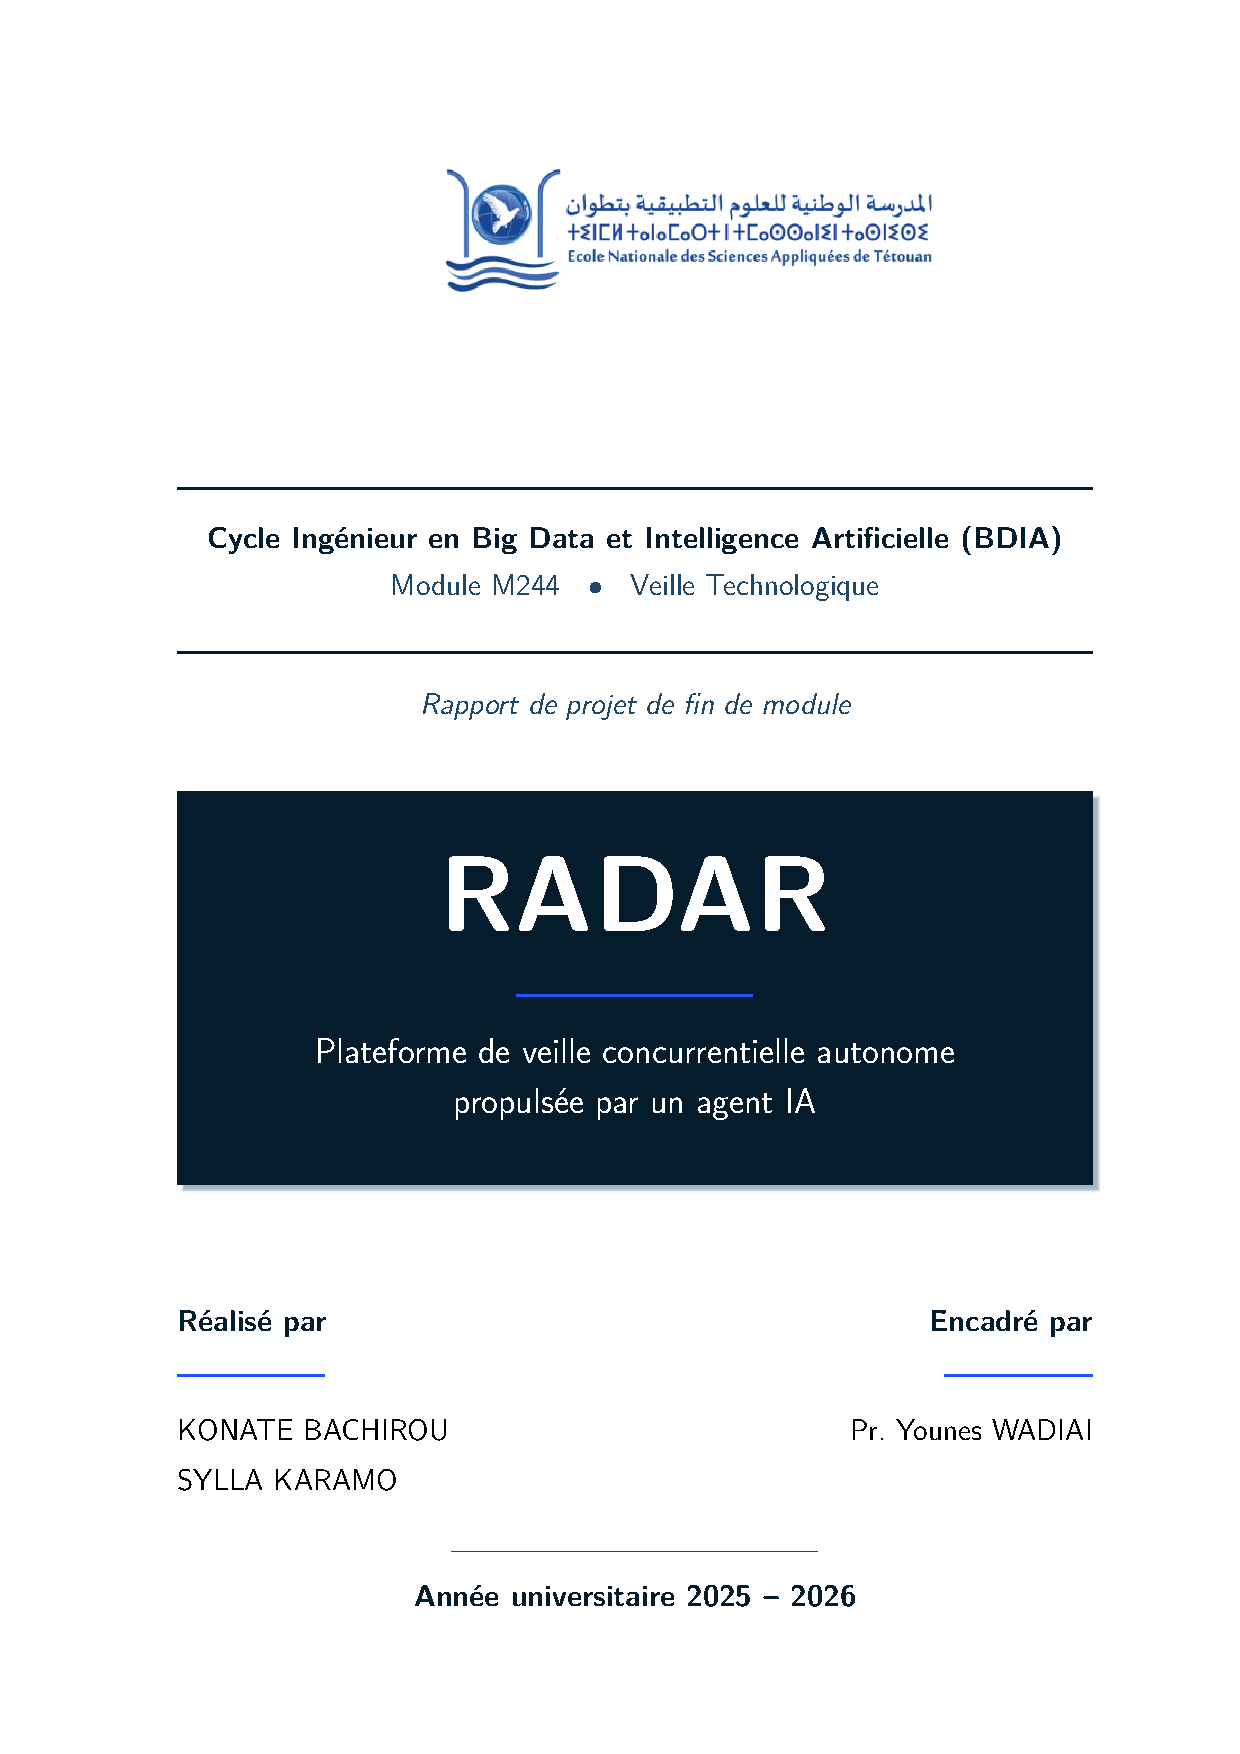
\includepdf[pages=-,fitpaper=true]{Rapport_technique_veille_projet_Radar.pdf}

\end{document}
